\section{Evaluation}

\begin{figure}[h]
    \centering
    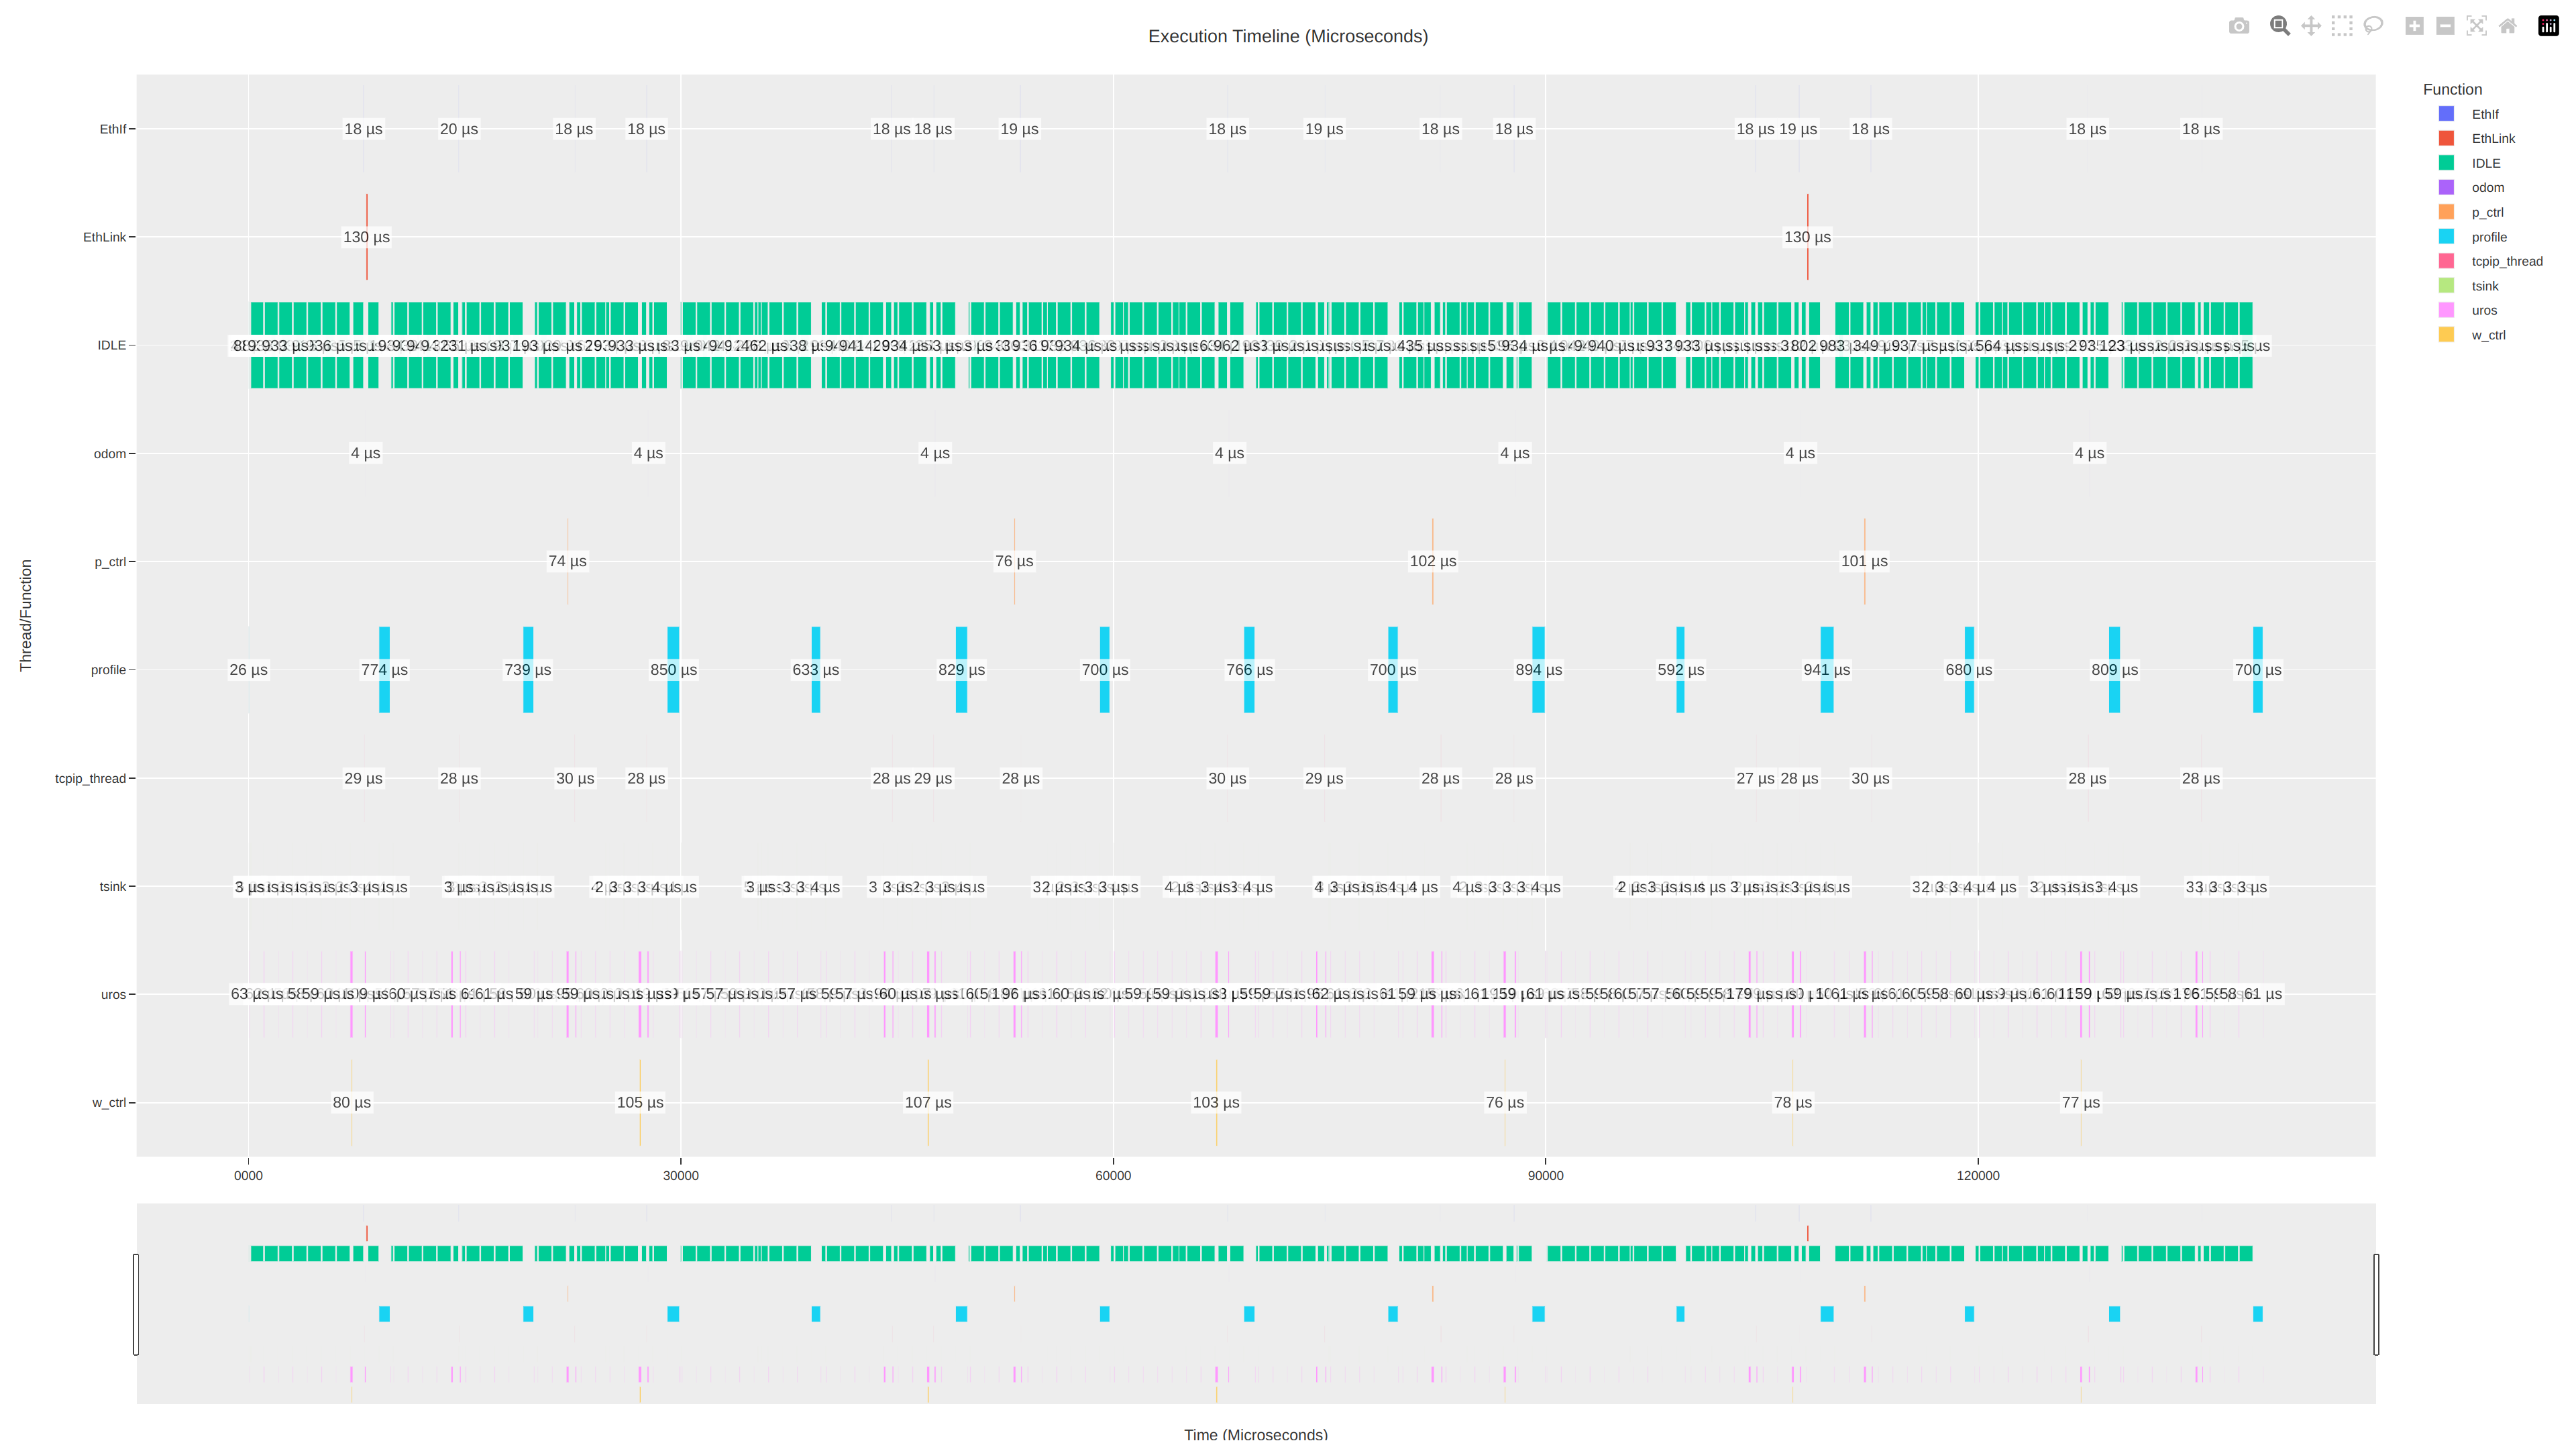
\includegraphics[width=1\textwidth]{assets/micro_ros_profiling}
    \caption{Visualisierung der Echtzeit-Statistik unter Micro-ROS}
    \label{fig:micro_ros_profiling}
\end{figure}

\begin{code}
\begin{minted}{cpp}
=======================================
free heap:          4688
ctx switches:       126810
Task            Time        %
profile         33450       2%
uros            106984      8%
IDLE            1179311     88%
EthLink         1695        <1%
tcpip_thread    4526        <1%
tsink           3762        <1%
Tmr Svc         0           <1%
EthIf           2730        <1%
---------------------------------------
Task        State   Prio    Stack   Num
uros            R     24     2548     3
profile         X     24     892      2
IDLE            R     0      108      4
tcpip_thread    B     24     180      6
tsink           B     32     475      1
EthLink         B     16     193      8
EthIf           B     48     17       7
Tmr Svc         B     2      223      5
=======================================
profiled for 18881864 us
\end{minted}
    \captionof{listing}{Zusammenfassung Echtzeitanalyse unter Micro-ROS}
    \label{code:freertos_summary_uros}
\end{code}

\begin{figure}[h]
    \centering
    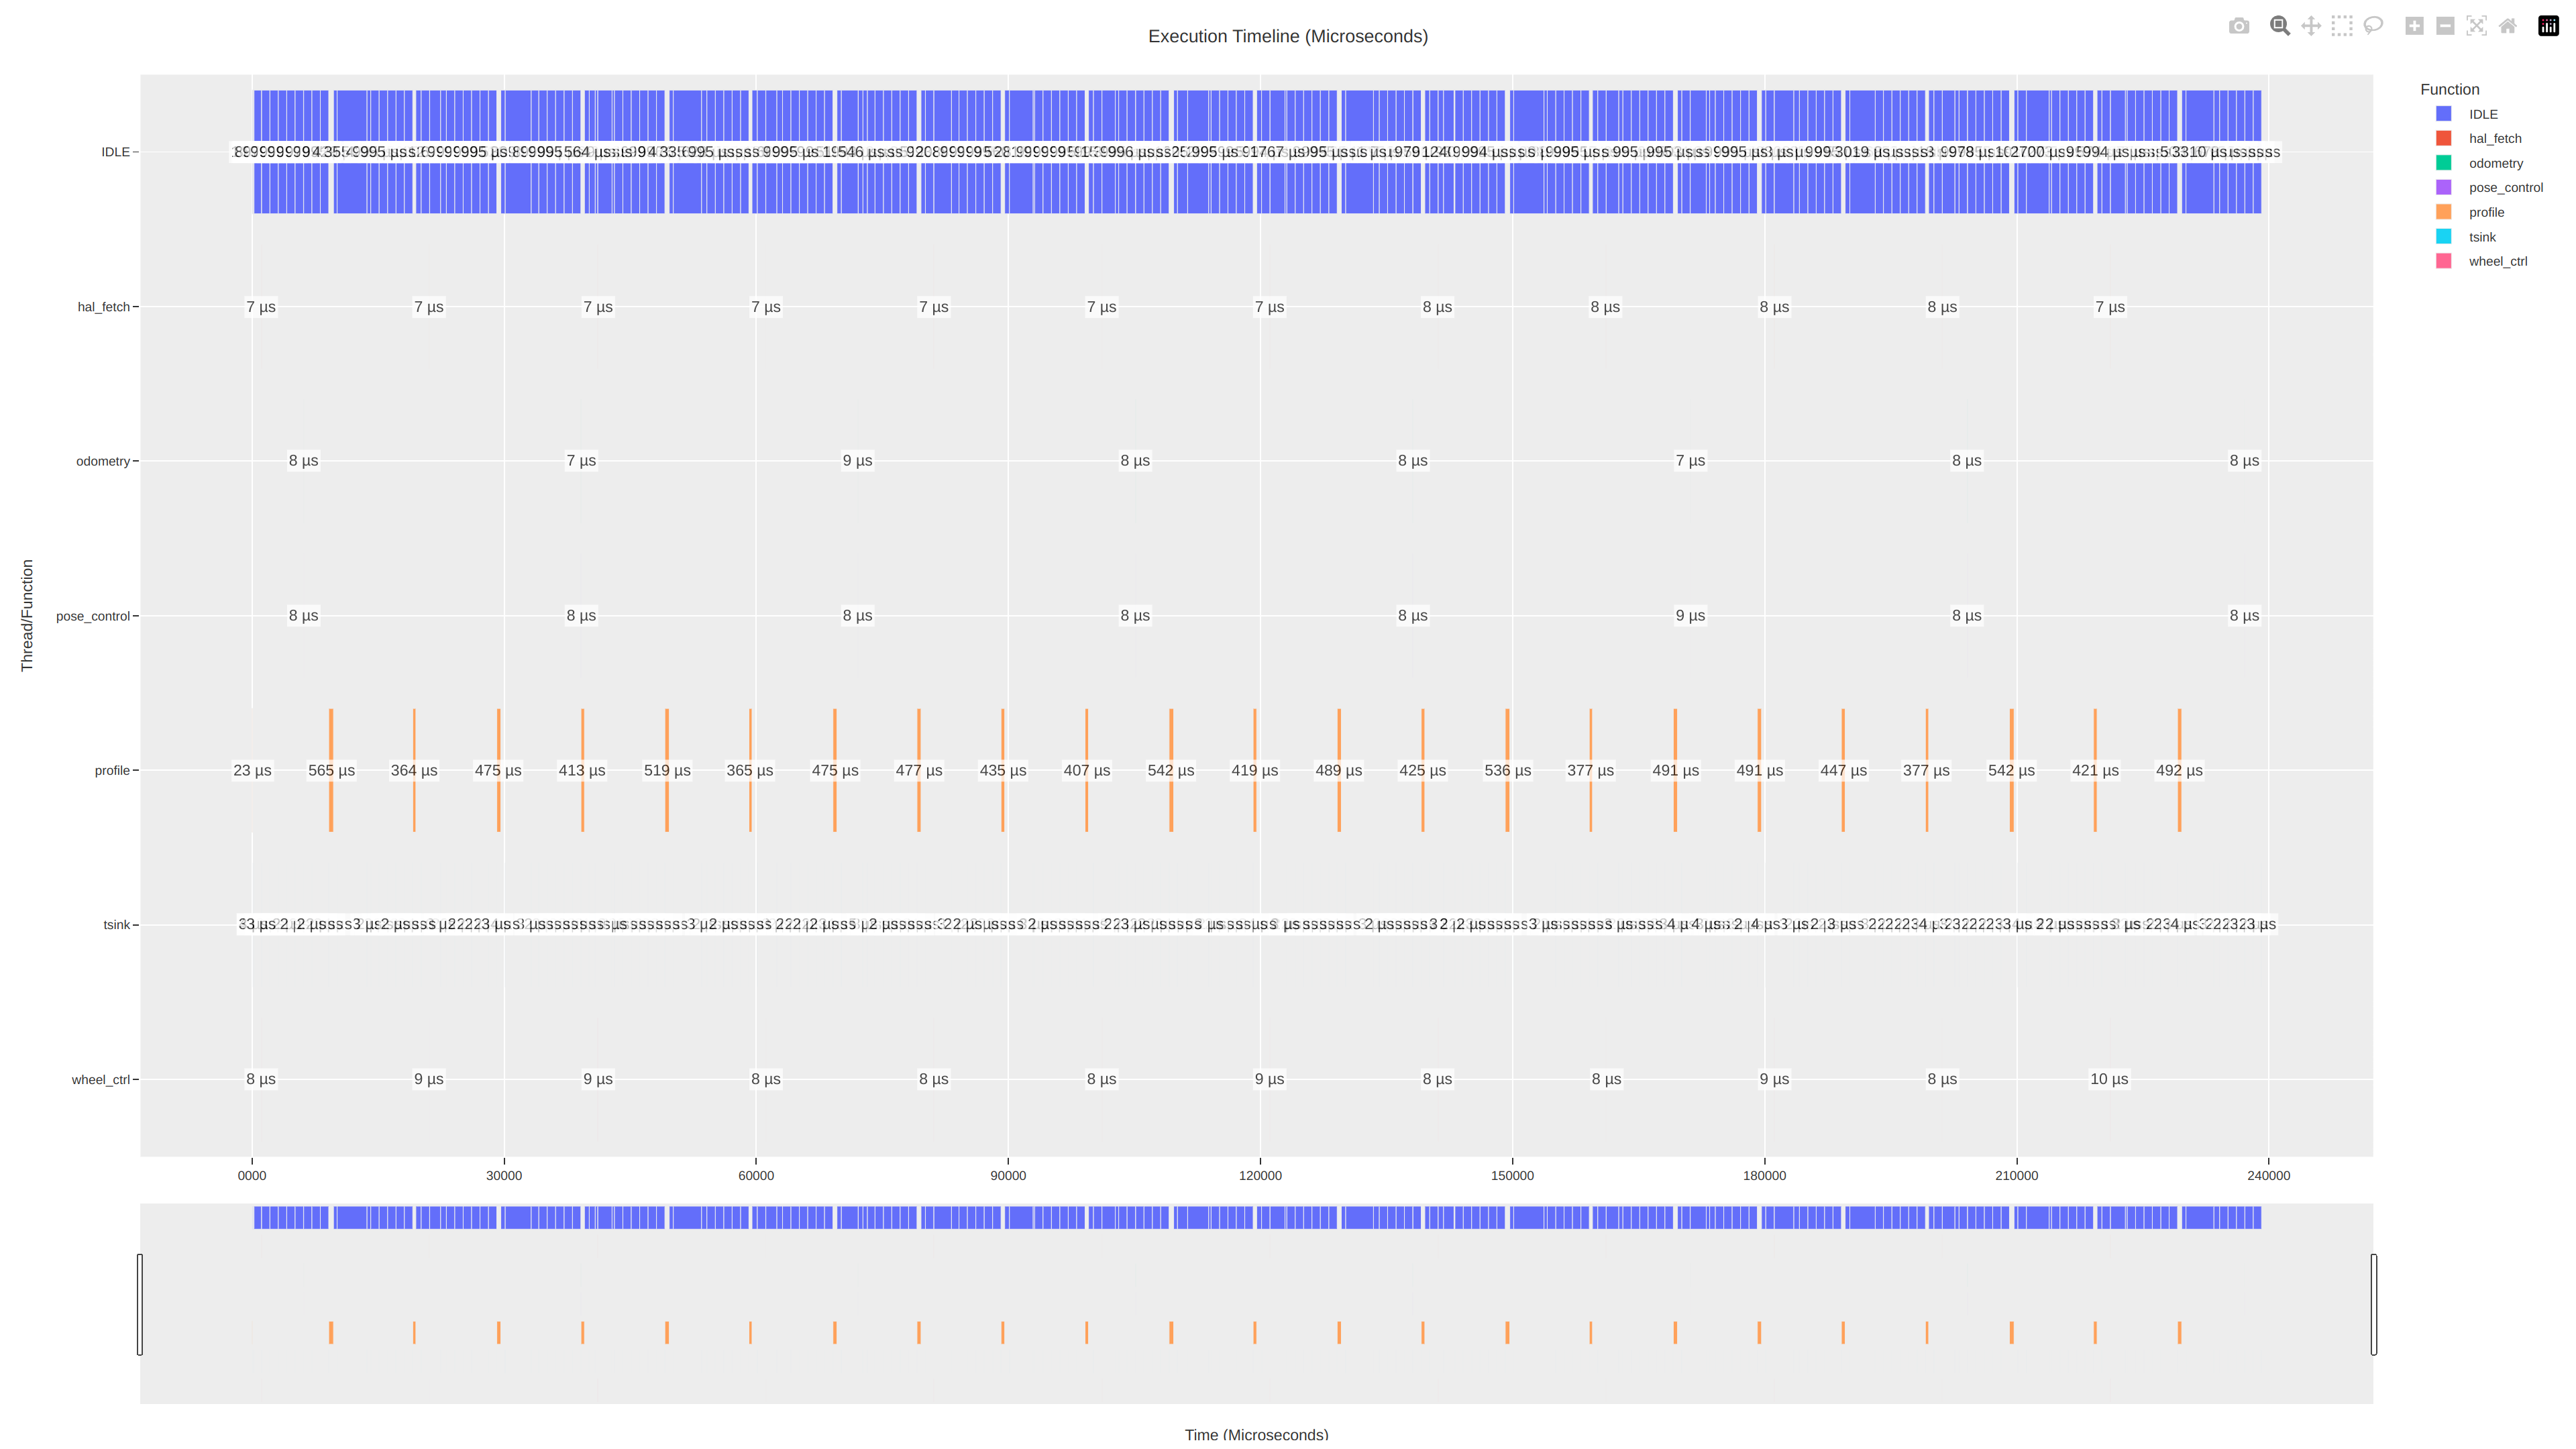
\includegraphics[width=1\textwidth]{assets/freertos_profiling}
    \caption{Visualisierung der Echtzeit-Statistik unter FreeRTOS}
    \label{fig:freertos_profiling}
\end{figure}

\begin{code}
\begin{minted}{cpp}
=======================================
free heap:          195696
ctx switches:       76148
Task            Time        %%
profile         9669        4%
IDLE            201086      95%
hal_fetch       81          <1%
wheel_ctrl      87          <1%
odometry        49          <1%
pose_control    51          <1%
tsink           615         <1%
Tmr Svc         0           <1%
recv_vel        0           <1%
---------------------------------------
Task        State   Prio    Stack   Num
profile         X      24     900     7
IDLE            R      0      108     8
wheel_ctrl      B      24     420     5
odometry        B      24     416     6
pose_control    B      24     410     4
tsink           B      32     483     1
hal_fetch       B      24     443     2
recv_vel        S      24     441     3
Tmr Svc         B      2      223     9
=======================================
profiled for 18779120 us
\end{minted}
    \captionof{listing}{Zusammenfassung Echtzeitanalyse unter FreeRTOS}
    \label{code:freertos_summary_freertos}
\end{code}

Die Profiling-Daten wurden mit einem Python-Skript verarbeitet und als
Gantt-Diagramm dargestellt (\ref{fig:freertos_profiling},
\ref{fig:micro_ros_profiling}). Dafür sortierte und aggregierte das Skript die
Start- und Endzeiten mittels der \mintinline{text}|pandas|-Bibliothek, bevor es
die Ergebnisse mittels \mintinline{text}|Plotly| visualisierte.

Am Ende eines Sampling-Vorgangs stellen die FreeRTOS-Funktionen
\mintinline{cpp}|vTaskGetRunTimeStats()| und \mintinline{cpp}|vTaskList()|
zusätzlich eine zusammenfassende Auswertung bereit
(\ref{code:freertos_summary_freertos}, \ref{code:freertos_summary_uros}), welche
die kumulierten Ausführungszeiten und Zustände aller Tasks vom Systemstart bis
zum Funktionsaufruf dokumentiert.

\begin{figure}[h]
    \centering
    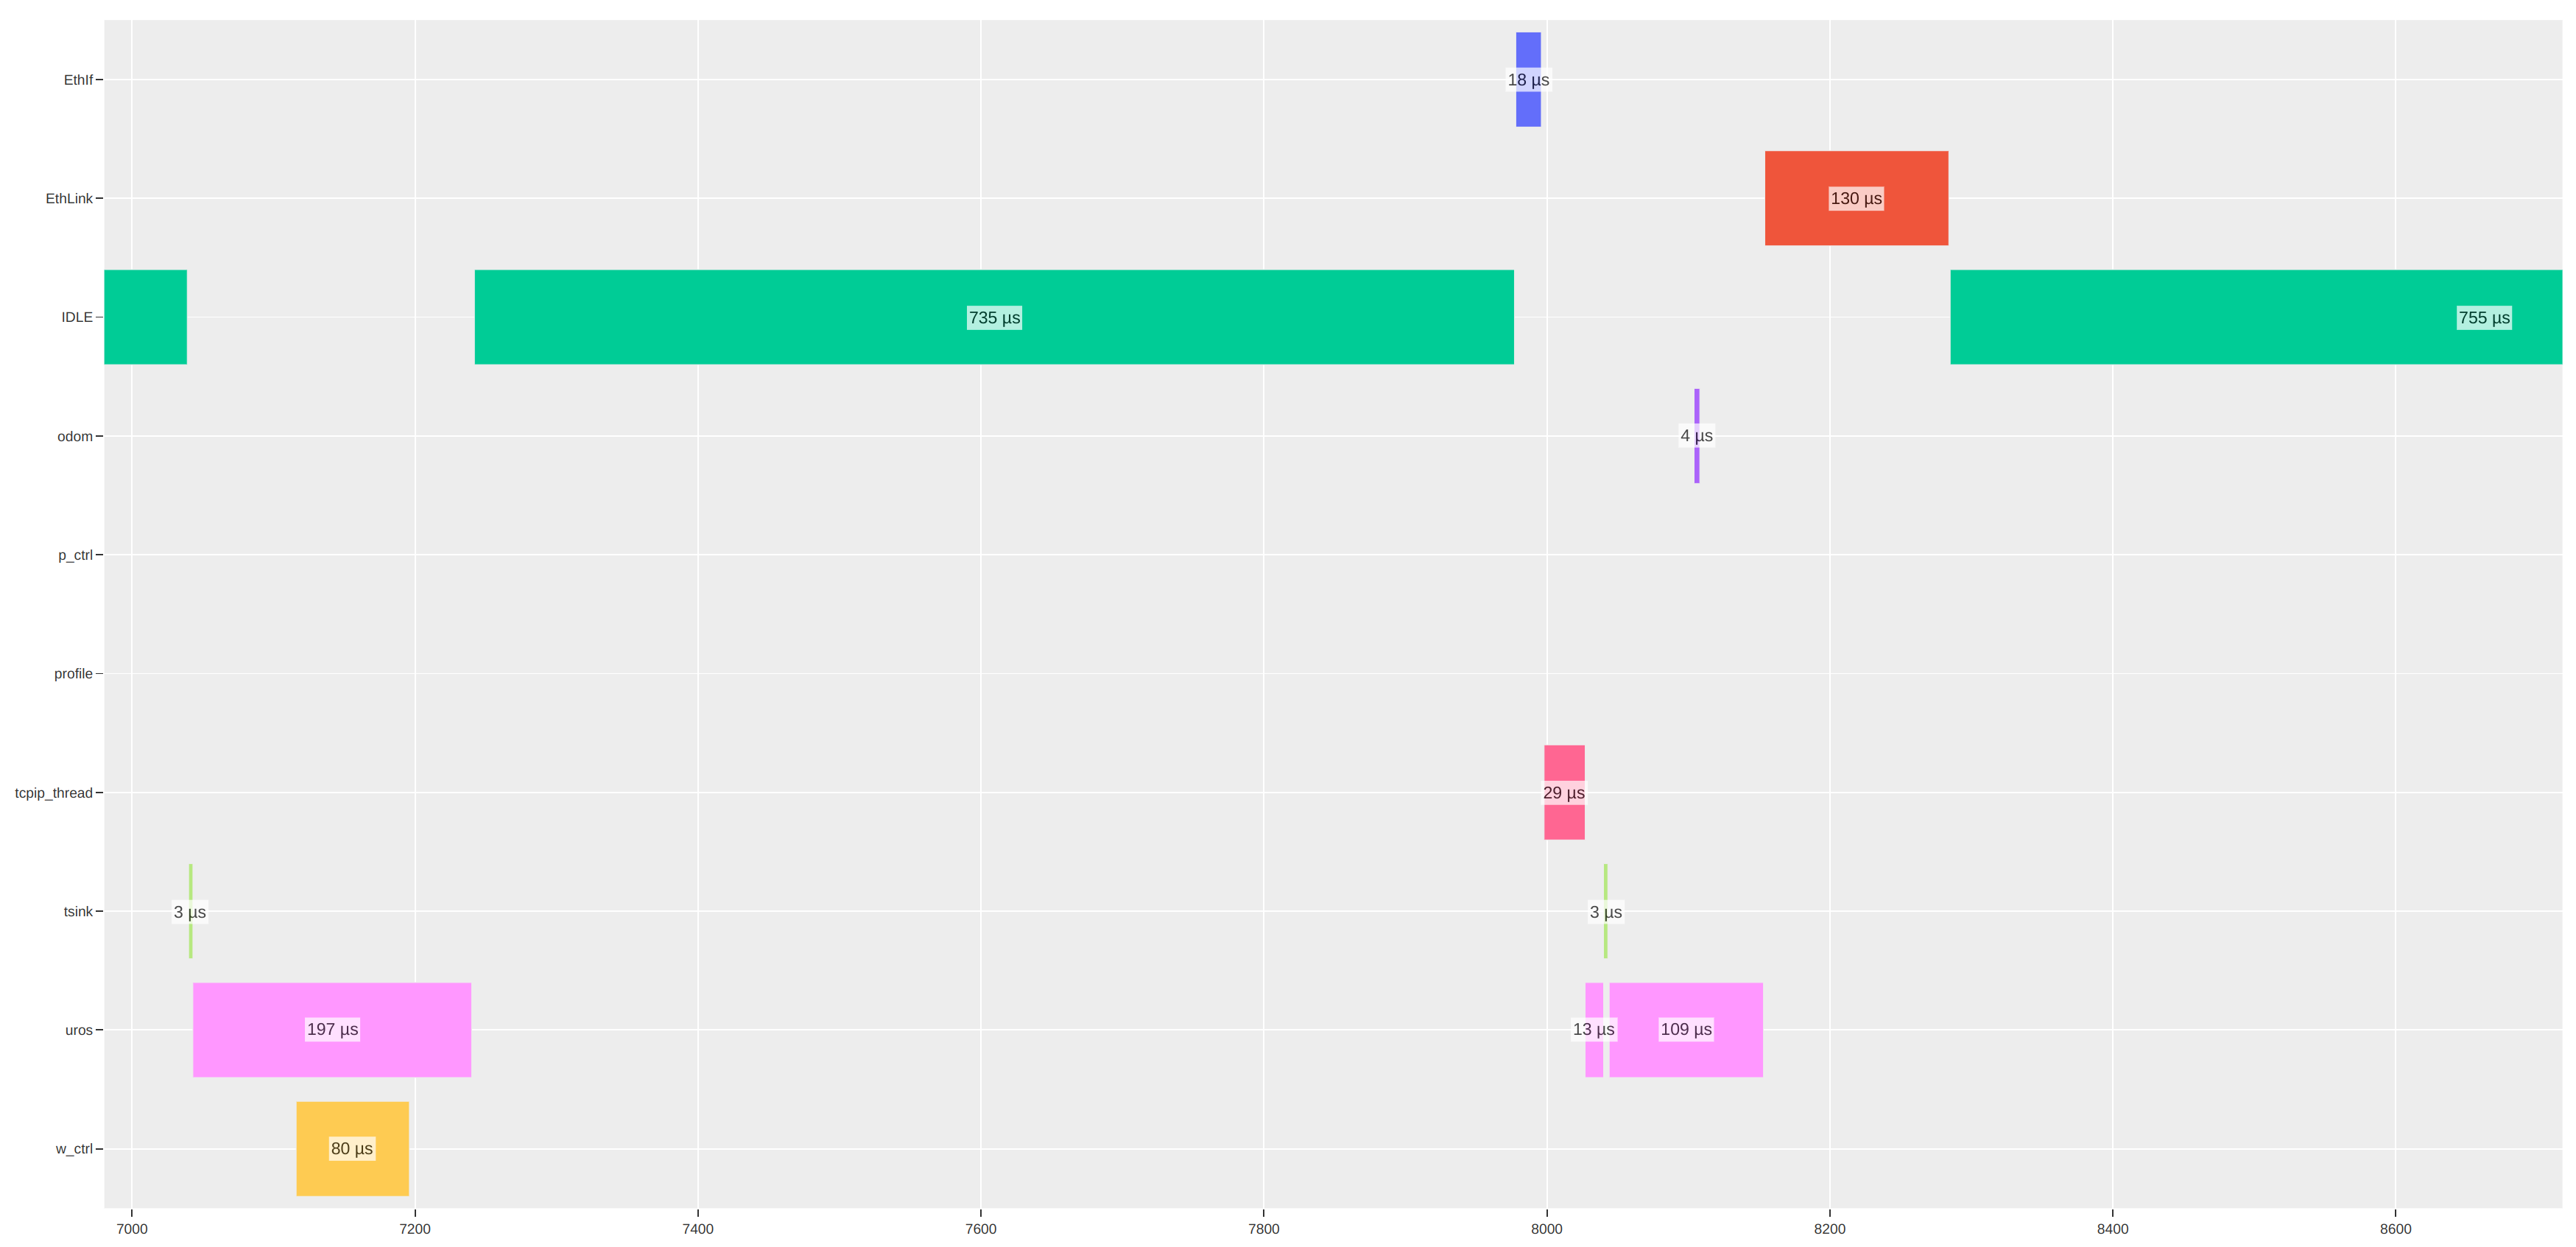
\includegraphics[width=1\textwidth]{assets/micro_ros_profiling_ausschnitt_cache_enabled}
    \caption{Visualisierung der Echtzeit-Statistik (Ausschnitt) unter Micro-ROS}
\end{figure}

\hyphenation{Low-Level-Da-ten-trans-port} Die Abbildung zeigt einen vergrößerten
Ausschnitt, der Kontextwechsel zwischen Tasks sowie Funktionsaufrufe
visualisiert. Während die gesamte Steuerungslogik innerhalb der Micro-ROS-Task
(\mintinline{text}|uros|) ausgeführt, arbeiten die Tasks unter anderem für den
zugrundeliegenden Datentransport, das Profiling und die Ausgabe parallel.

\subsection{Laufzeit-Statistik -- Micro-ROS}

\subsubsection{Regler mit 50 Hz und 30 Hz}

Bei einer Sollfrequenz von $50\,\text{Hz}$ für die Drehzahlregelung und
$30\,\text{Hz}$ für die Positionsregelung mit Odometrie zeigen die
Messergebnisse nach etwa $18$ Sekunden Profiling folgende Werte -- jeweils ohne
und mit Cache:

\begin{table}[H]
\centering
\small
\setlength{\tabcolsep}{4pt}
\makebox[0pt][c]{\parbox{1.1\textwidth} \\ \hline
        \mintinline{text}|EthIf| & 52,93 & 115.022 & 0,62\,\% \\ \hline
        \mintinline{text}|EthLink| & 128,38 & 26.702 & 0,14\,\% \\ \hline
        \mintinline{text}|IDLE| & 587,79 & 8.961.378 & \textbf{48,17\,\%} \\ \hline
        \mintinline{text}|odom| & 8,88 & 8.186 & \textbf{0,04\,\%} \\ \hline
        \mintinline{text}|p_ctrl| & 277,97 & 170.671 & \textbf{0,92\,\%} \\ \hline
        \mintinline{text}|profile| & 623,40 & 4.981.587 & 26,78\,\% \\ \hline
        \mintinline{text}|tcpip_thread| & 71,16 & 176.607 & 0,95\,\% \\ \hline
        \mintinline{text}|tsink| & 8,80 & 120.659 & 0,65\,\% \\ \hline
        \mintinline{text}|uros| & 203,31 & 3.807.442 & \textbf{20,47\,\%} \\ \hline
        \mintinline{text}|w_ctrl| & 256,11 & 236.136 & \textbf{1,27\,\%} \\ \hline
        \hline
        \textbf{Summe} & - & 18.604.390 & 100,00\,\% \\ \hline
        \end{tabular}
        \caption{Laufzeit-Statistik ohne Caching}
    \end{minipage}
    \hfill
    \begin{minipage}[b]{0.50\hsize}\centering
        \begin{tabular}{|l|r|r|r|}
        \hline
        \textbf{Name}  & \textbf{Ø (µs)} & \textbf{Summe} & \textbf{\%} \\ \hline
        \mintinline{text}|EthIf| & 18,43 & 40.671 & 0,21\,\% \\ \hline
        \mintinline{text}|EthLink| & 123,53 & 24.583 & 0,13\,\% \\ \hline
        \mintinline{text}|IDLE| & 661,14 & 15.505.748 & \textbf{81,81\,\%} \\ \hline
        \mintinline{text}|odom| & 4,02 & 3.791 & \textbf{0,02\,\%} \\ \hline
        \mintinline{text}|p_ctrl| & 88,25 & 55.511 & \textbf{0,29\,\%} \\ \hline
        \mintinline{text}|profile| & 803,55 & 1.517.905 & 8,01\,\% \\ \hline
        \mintinline{text}|tcpip_thread| & 28,29 & 63.613 & 0,34\,\% \\ \hline
        \mintinline{text}|tsink| & 3,37 & 41.113 & 0,22\,\% \\ \hline
        \mintinline{text}|uros| & 76,17 & 1.614.854 & \textbf{8,52\,\%} \\ \hline
        \mintinline{text}|w_ctrl| & 90,82 & 85.646 & \textbf{0,45\,\%} \\ \hline
        \hline
        \textbf{Summe} & - & 18.953.435 & 100,00\,\% \\ \hline
        \end{tabular}
        \caption{Laufzeit-Statistik mit Caching}
    \end{minipage}
}}
\end{table}

\subsubsection{Regler mit 100 Hz und 50 Hz}

Bei einer Sollfrequenz von $100\,\text{Hz}$ für die Drehzahlregelung und
$50\,\text{Hz}$ für die Positionsregelung mit Odometrie zeigen die
Messergebnisse nach etwa $18$ Sekunden Profiling folgende Werte -- jeweils ohne
und mit Cache:

\begin{table}[H]
\centering
\small
\setlength{\tabcolsep}{4pt}
\makebox[0pt][c]{\parbox{1.1\textwidth} \\ \hline
        \mintinline{text}|EthIf| & 51,53 & 198.643 & 1,05\,\% \\ \hline
        \mintinline{text}|EthLink| & 110,25 & 26.130 & 0,14\,\% \\ \hline
        \mintinline{text}|IDLE| & 545,36 & 7.330.732 & \textbf{38,75\,\%} \\ \hline
        \mintinline{text}|odom| & 9,92 & 18.149 & \textbf{0,10\,\%} \\ \hline
        \mintinline{text}|p_ctrl| & 322,41 & 295.008 & \textbf{1,56\,\%} \\ \hline
        \mintinline{text}|profile| & 566,25 & 5.472.282 & 28,92\,\% \\ \hline
        \mintinline{text}|tcpip_thread| & 71,13 & 296.128 & 1,57\,\% \\ \hline
        \mintinline{text}|tsink| & 8,80 & 113.096 & 0,60\,\% \\ \hline
        \mintinline{text}|uros| & 231,74 & 4.606.256 & \textbf{24,35\,\%} \\ \hline
        \mintinline{text}|w_ctrl| & 307,53 & 562.785 & \textbf{2,97\,\%} \\ \hline
        \hline
        \textbf{Summe} & -- & 18.919.209 & 100,00\,\% \\ \hline
        \end{tabular}
        \caption{Laufzeit-Statistik ohne Caching}
    \end{minipage}
    \hfill
    \begin{minipage}[b]{0.50\hsize}\centering
        \begin{tabular}{|l|r|r|r|}
        \hline
        \textbf{Name}  & \textbf{Ø (µs)} & \textbf{Summe} & \textbf{\%} \\ \hline
        \mintinline{text}|EthIf| & 18,81 & 68.712 & 0,37\,\% \\ \hline
        \mintinline{text}|EthLink| & 128,88 & 23.971 & 0,13\,\% \\ \hline
        \mintinline{text}|IDLE| & 607,96 & 14.540.662 & \textbf{78,00\,\%} \\ \hline
        \mintinline{text}|odom| & 3,74 & 6.780 & \textbf{0,04\,\%} \\ \hline
        \mintinline{text}|p_ctrl| & 75,16 & 69.301 & \textbf{0,37\,\%} \\ \hline
        \mintinline{text}|profile| & 889,48 & 1.641.972 & 8,81\,\% \\ \hline
        \mintinline{text}|tcpip_thread| & 28,25 & 104.623 & 0,56\,\% \\ \hline
        \mintinline{text}|tsink| & 3,43 & 36.583 & 0,20\,\% \\ \hline
        \mintinline{text}|uros| & 86,44 & 1.957.616 & \textbf{10,50\,\%} \\ \hline
        \mintinline{text}|w_ctrl| & 103,59 & 191.027 & \textbf{1,02\,\%} \\ \hline
        \hline
        \textbf{Summe} & -- & 18.641.247 & 100,00\,\% \\ \hline
        \end{tabular}
        \caption{Laufzeit-Statistik mit Caching}
    \end{minipage}
}}
\end{table}

Ohne Daten- oder Instruktionscache benötigte die Micro-ROS-Task für die gesamte
Steuerungslogik bei den Reglern mit $50\,\text{Hz}$ sowie $30\,\text{Hz}$
$\textbf{20,47\,\%}$ Rechenzeit. Bei $100\,\text{Hz}$ sowie $50\,\text{Hz}$
waren es $\textbf{24,35\,\%}$. Gleichzeitig befand sich das System zu
$\textbf{48,17\,\%}$ bzw. $\textbf{38,75\,\%}$ im Leerlauf.

Mit aktiviertem Daten- und Instruktionscache benötigte die Micro-ROS-Task bei
den Reglern mit $50\,\text{Hz}$ sowie $30\,\text{Hz}$ nur $\textbf{8,52\,\%}$
Rechenzeit. Bei höheren Frequenzen ($100\,\text{Hz}$ sowie $50\,\text{Hz}$) sind
es $\textbf{10,50\,\%}$, während die Leerlaufzeit bei $\textbf{81,81\,\%}$ bzw.
$\textbf{78,00\,\%}$ liegt.

Durch die Aktivierung der Caches reduzierte sich die akkumulierte Rechenzeit
beispielsweise in der $100\,\text{Hz}/50\,\text{Hz}$-Reglerkonfiguration
deutlich: um $\textbf{62,64\,\%}$ für die Odometrie, $\textbf{76,51\,\%}$ für
die Posenregelung und $\textbf{66,06\,\%}$ für die Drehzahlregelung.
Gleichzeitig stiegen die Leerlaufzeiten um $\textbf{98,35\,\%}$ an, wobei die
gesamte Profiling-Dauer zwischen den beiden Sampling-Vorgangs eine Differenz von
$349,\!045\,\text{ms}$ aufwies.

\subsection{Laufzeit-Statistik -- FreeRTOS}

\subsubsection{Regler mit 50 Hz und 30 Hz}

\begin{table}[H]
\centering
\small
\setlength{\tabcolsep}{4pt}
\makebox[0pt][c]{\parbox{1.1\textwidth} \\ \hline
        \mintinline{text}|IDLE| & 983,50 & 14.996.422 & \textbf{81,85\%} \\ \hline
        \mintinline{text}|hal_fetch| & 21,71 & 20.403 & 0,11\% \\ \hline
        \mintinline{text}|odometry| & 24,05 & 13.634 & \textbf{0,07\%} \\ \hline
        \mintinline{text}|pose_control| & 32,66 & 18.682 & \textbf{0,10\%} \\ \hline
        \mintinline{text}|profile| & 902,87 & 3.077.879 & 16,80\% \\ \hline
        \mintinline{text}|tsink| & 9,63 & 161.451 & 0,88\% \\ \hline
        \mintinline{text}|wheel_ctrl| & 35,80 & 34.260 & \textbf{0,19\%} \\ \hline
        \hline
        \textbf{Summe} & -- & 18.322.731 & 100,00\,\% \\ \hline
        \end{tabular}
        \caption{Laufzeit-Statistik ohne Caching}
    \end{minipage}
    \hfill
    \begin{minipage}[b]{0.50\hsize}\centering
        \begin{tabular}{|l|r|r|r|}
        \hline
        \textbf{Name}  & \textbf{Ø (µs)} & \textbf{Summe} & \textbf{\%} \\ \hline
        \mintinline{text}|IDLE| & 1.041,06 & 17.658.382 & \textbf{94,83\,\%} \\ \hline
        \mintinline{text}|hal_fetch| & 6,43 & 6.003 & 0,03\,\% \\ \hline
        \mintinline{text}|odometry| & 7,19 & 4.068 & \textbf{0,02\,\%} \\ \hline
        \mintinline{text}|pose_control| & 9,64 & 5.456 & \textbf{0,03\,\%} \\ \hline
        \mintinline{text}|profile| & 476,43 & 889.027 & 4,77\,\% \\ \hline
        \mintinline{text}|tsink| & 2,95 & 46.947 & 0,25\,\% \\ \hline
        \mintinline{text}|wheel_ctrl| & 10,96 & 10.379 & \textbf{0,06\,\%} \\ \hline
        \hline
        \textbf{Summe} & -- & 18.620.262 & 100,00\,\% \\ \hline
        \end{tabular}
        \caption{Laufzeit-Statistik mit Caching}
    \end{minipage}
}}
\end{table}

\subsubsection{Regler mit 100 Hz und 50 Hz}

\begin{table}[H]
\centering
\small
\setlength{\tabcolsep}{4pt}
\makebox[0pt][c]{\parbox{1.1\textwidth} \\ \hline
        \mintinline{text}|IDLE| & 997,02 & 14.706.086 & \textbf{80,67\,\%} \\ \hline
        \mintinline{text}|hal_fetch| & 21,91 & 40.471 & 0,22\,\% \\ \hline
        \mintinline{text}|odometry| & 24,01 & 22.373 & \textbf{0,12\,\%} \\ \hline
        \mintinline{text}|pose_control| & 32,46 & 30.579 & \textbf{0,17\,\%} \\ \hline
        \mintinline{text}|profile| & 941,93 & 3.209.167 & 17,60\,\% \\ \hline
        \mintinline{text}|tsink| & 9,36 & 151.046 & 0,83\,\% \\ \hline
        \mintinline{text}|wheel_ctrl| & 37,77 & 70.285 & \textbf{0,39\,\%} \\ \hline
        \hline
        \textbf{Summe} & {--} & 18.230.007 & 100,00\,\% \\ \hline
        \end{tabular}
        \caption{Laufzeit-Statistik ohne Caching}
    \end{minipage}
    \hfill
    \begin{minipage}[b]{0.50\hsize}\centering
        \begin{tabular}{|l|r|r|r|}
        \hline
        \textbf{Name}  & \textbf{Ø (µs)} & \textbf{Summe} & \textbf{\%} \\ \hline
        \mintinline{text}|IDLE| & 1.139,87 & 17.276.974 & \textbf{94,61\,\%} \\ \hline
        \mintinline{text}|hal_fetch| & 6,61 & 12.104 & 0,07\,\% \\ \hline
        \mintinline{text}|odometry| & 6,84 & 6.256 & \textbf{0,03\,\%} \\ \hline
        \mintinline{text}|pose_control| & 9,88 & 9.043 & \textbf{0,05\,\%} \\ \hline
        \mintinline{text}|profile| & 487,57 & 892.246 & 4,89\,\% \\ \hline
        \mintinline{text}|tsink| & 3,01 & 45.597 & 0,25\,\% \\ \hline
        \mintinline{text}|wheel_ctrl| & 10,69 & 19.559 & \textbf{0,11\,\%} \\ \hline
        \hline
        \textbf{Summe} & {--} & 18.443.591 & 100.00\,\% \\ \hline
        \end{tabular}
        \caption{Laufzeit-Statistik mit Caching}
    \end{minipage}
}}
\end{table}

Ohne Micro-ROS-Abhängigkeit erreicht das System bereits ohne Caches eine
Leerlaufzeit von etwa $\textbf{80\,\%}$. Mit aktivierten Caches steigt diese auf
circa $\textbf{95\,\%}$ an.


Die Performance-Steigerung durch das Aktivieren der Caches ist bei der
FreeRTOS-Implementierung ebenfalls signifikant, wobei sich die gesamte
Profiling-Dauer beider Samplings bei der
$100\,\text{Hz}|50\,\text{Hz}$-Reglerkonfiguration um $213,584\,\text{ms}$
unterscheidet. Die Rechenzeiten verringerten sich für die Odometrie um
$\textbf{72,04\,\%}$, für die Posenregelung um $\textbf{70,43\,\%}$ sowie für
die Drehzahlregelung um $\textbf{72,17\,\%}$. Die Leerlaufzeit stieg dabei um
$\textbf{14,88\,\%}$, 

\subsection{Vergleich zwischen Micro-ROS und FreeRTOS}

\subsubsection{Experimentelle Bestimmung der maximalen Regelungsfrequenz}

Bei FreeRTOS gibt es keine theoretische Obergrenze für die Taktfrequenz von
Tasks. Die praktische maximale Frequenz liegt standardmäßig bei
$1000\,\text{Hz}$, da der Tick-Interrupt für den Kontextwechsel standardmäßig
auf $1\,\text{ms}$ (entsprechend $1000$ Interrupts pro Sekunde) festgelegt ist
\cite{FreertosTasks}.

Um Frequenzen über $1000\,\text{Hz}$ zu erreichen, müsste die
Tick-Interrupt-Frequenz angepasst werden, um die Zeitscheibenlänge (time slice)
zwischen den Interrupts zu reduzieren. Von Frequenzen über 1000 Hz wird jedoch
abgeraten, da die kumulativen Kontextwechselkosten einen spürbaren Overhead
verursachen \cite{FreertosTickRate2010}. Für hochfrequente Aufgaben empfiehlt
sich daher der Verzicht auf ein RTOS zugunsten eines minimalen
Scheduling-Verfahrens \cite{FreertosForumHF2019}.

\begin{figure}[H]
    \centering
    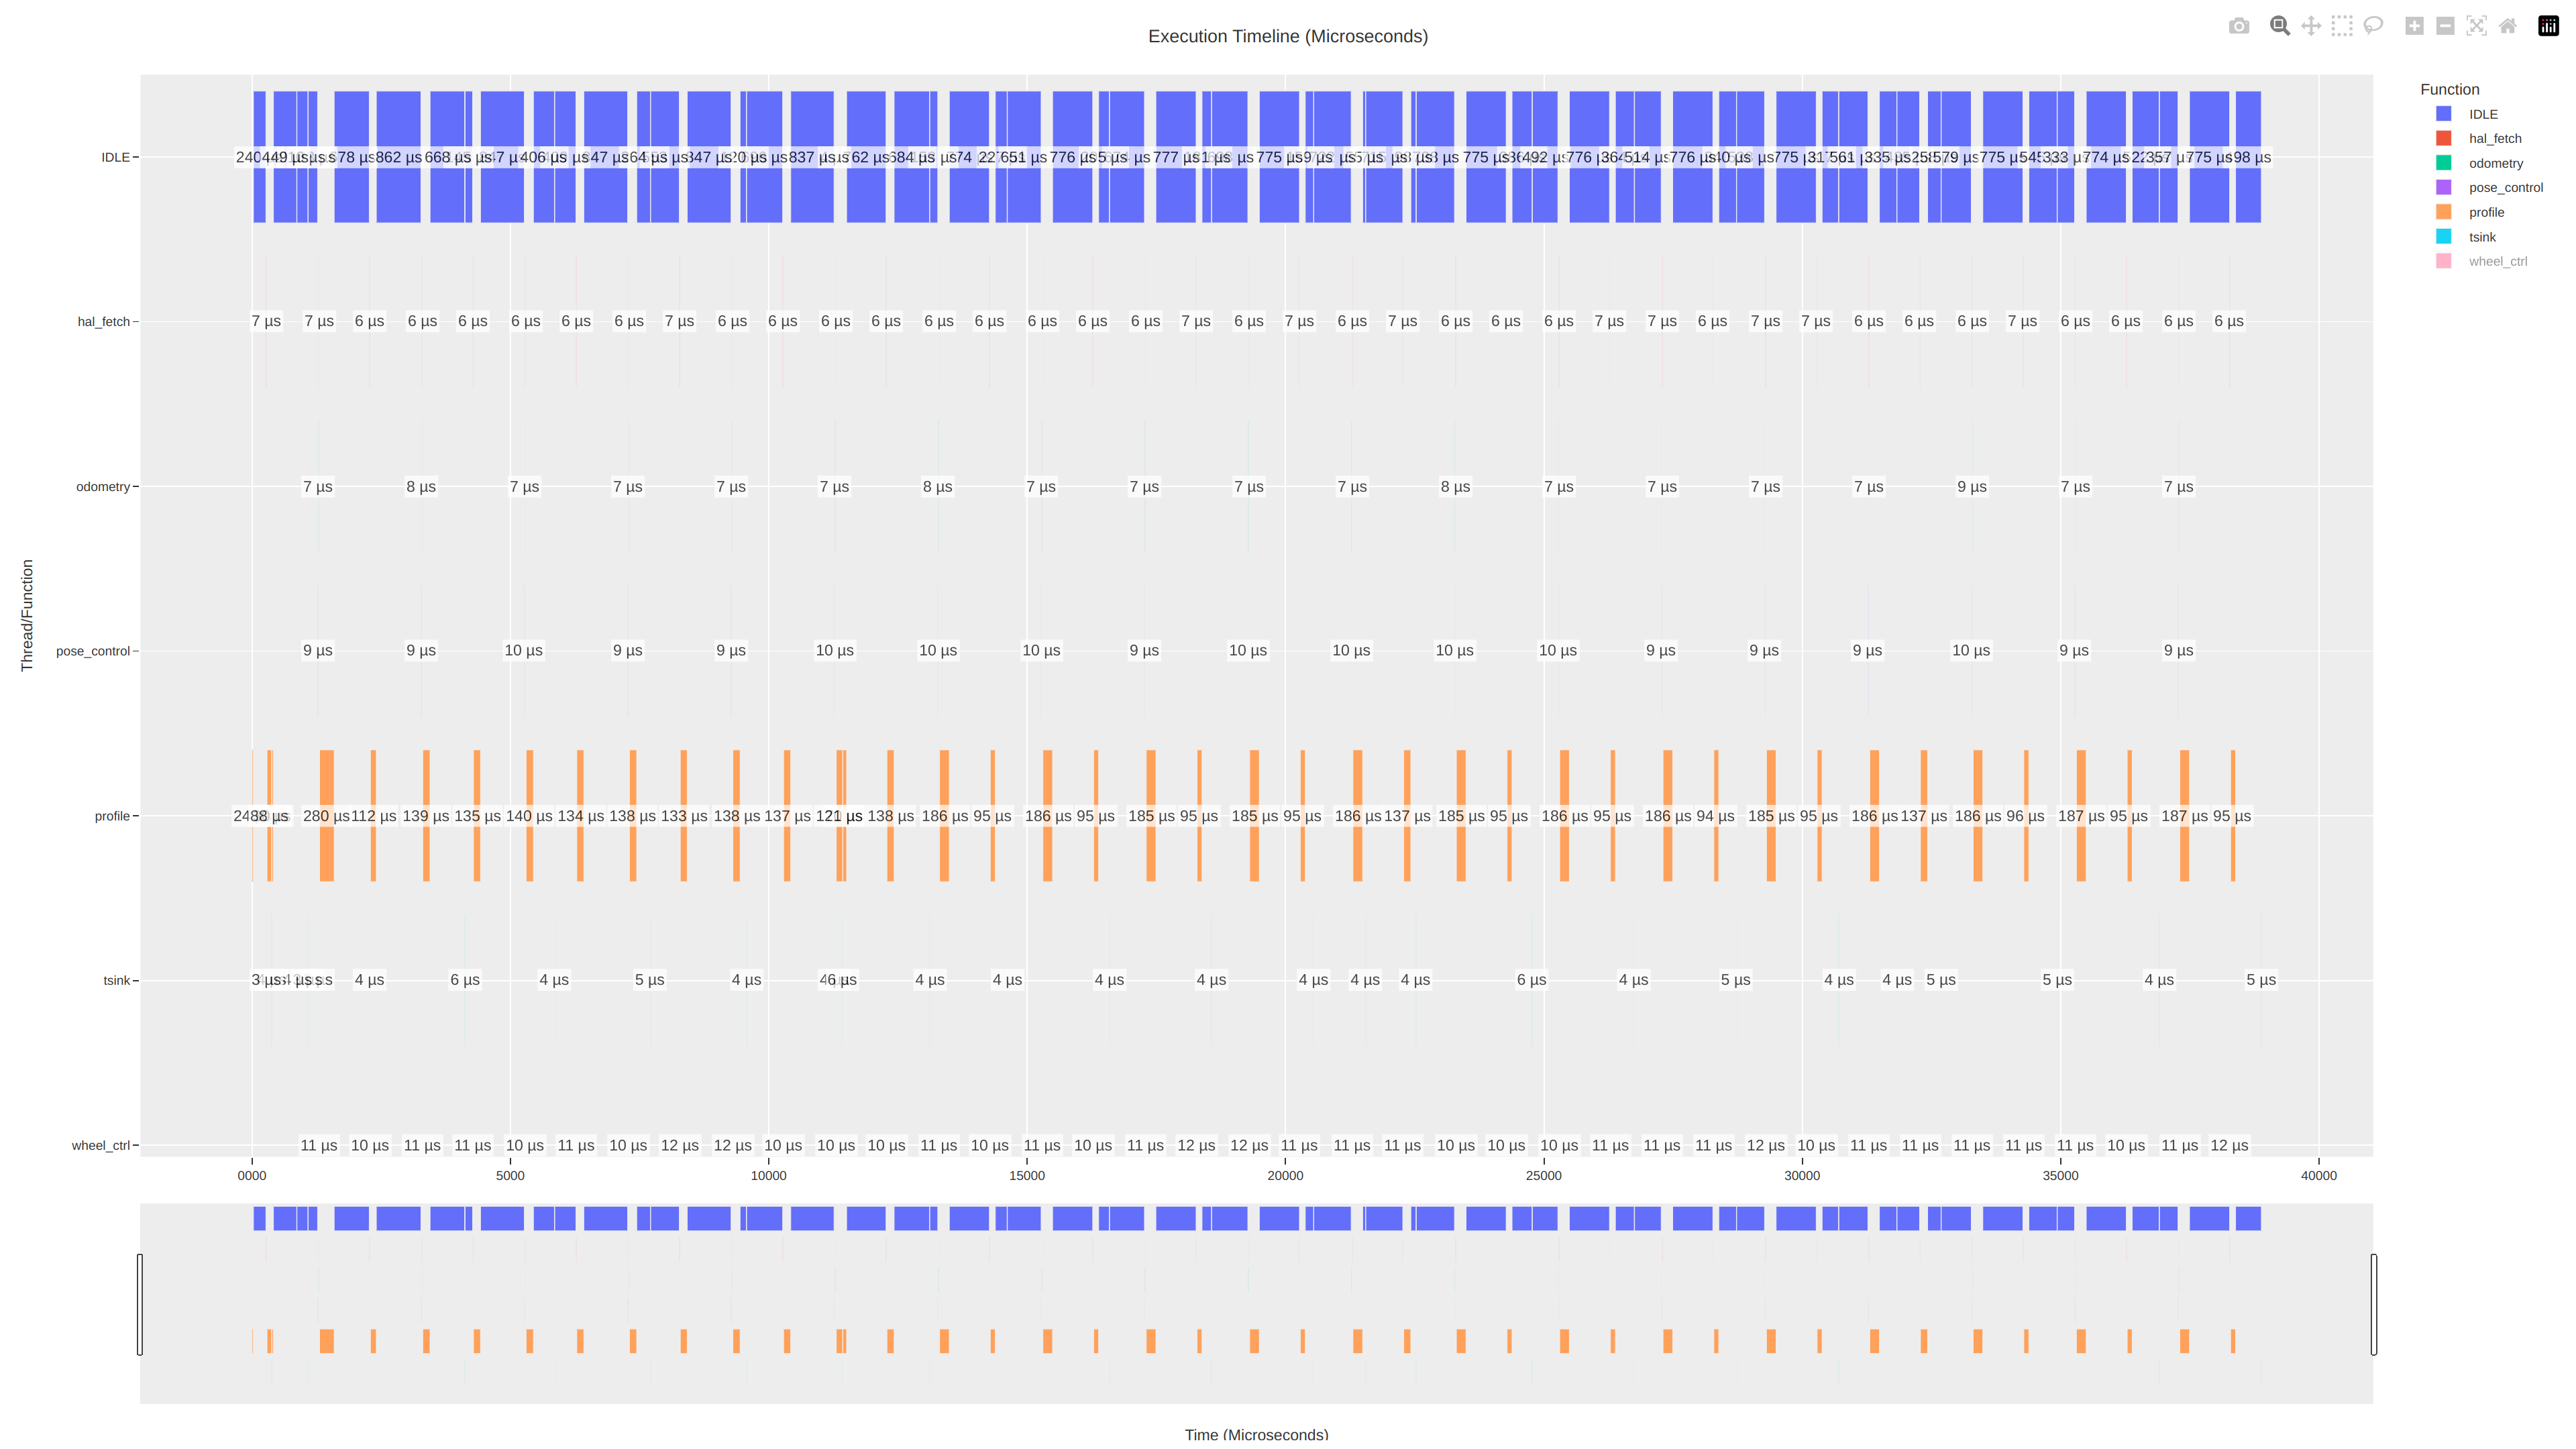
\includegraphics[width=1\textwidth]{assets/freertos_profiling_1000hz}
    \caption{Visualisierung der Echtzeit-Statistik mit 1000 Hz unter FreeRTOS}
\end{figure}

\begin{figure}[H]
    \centering
    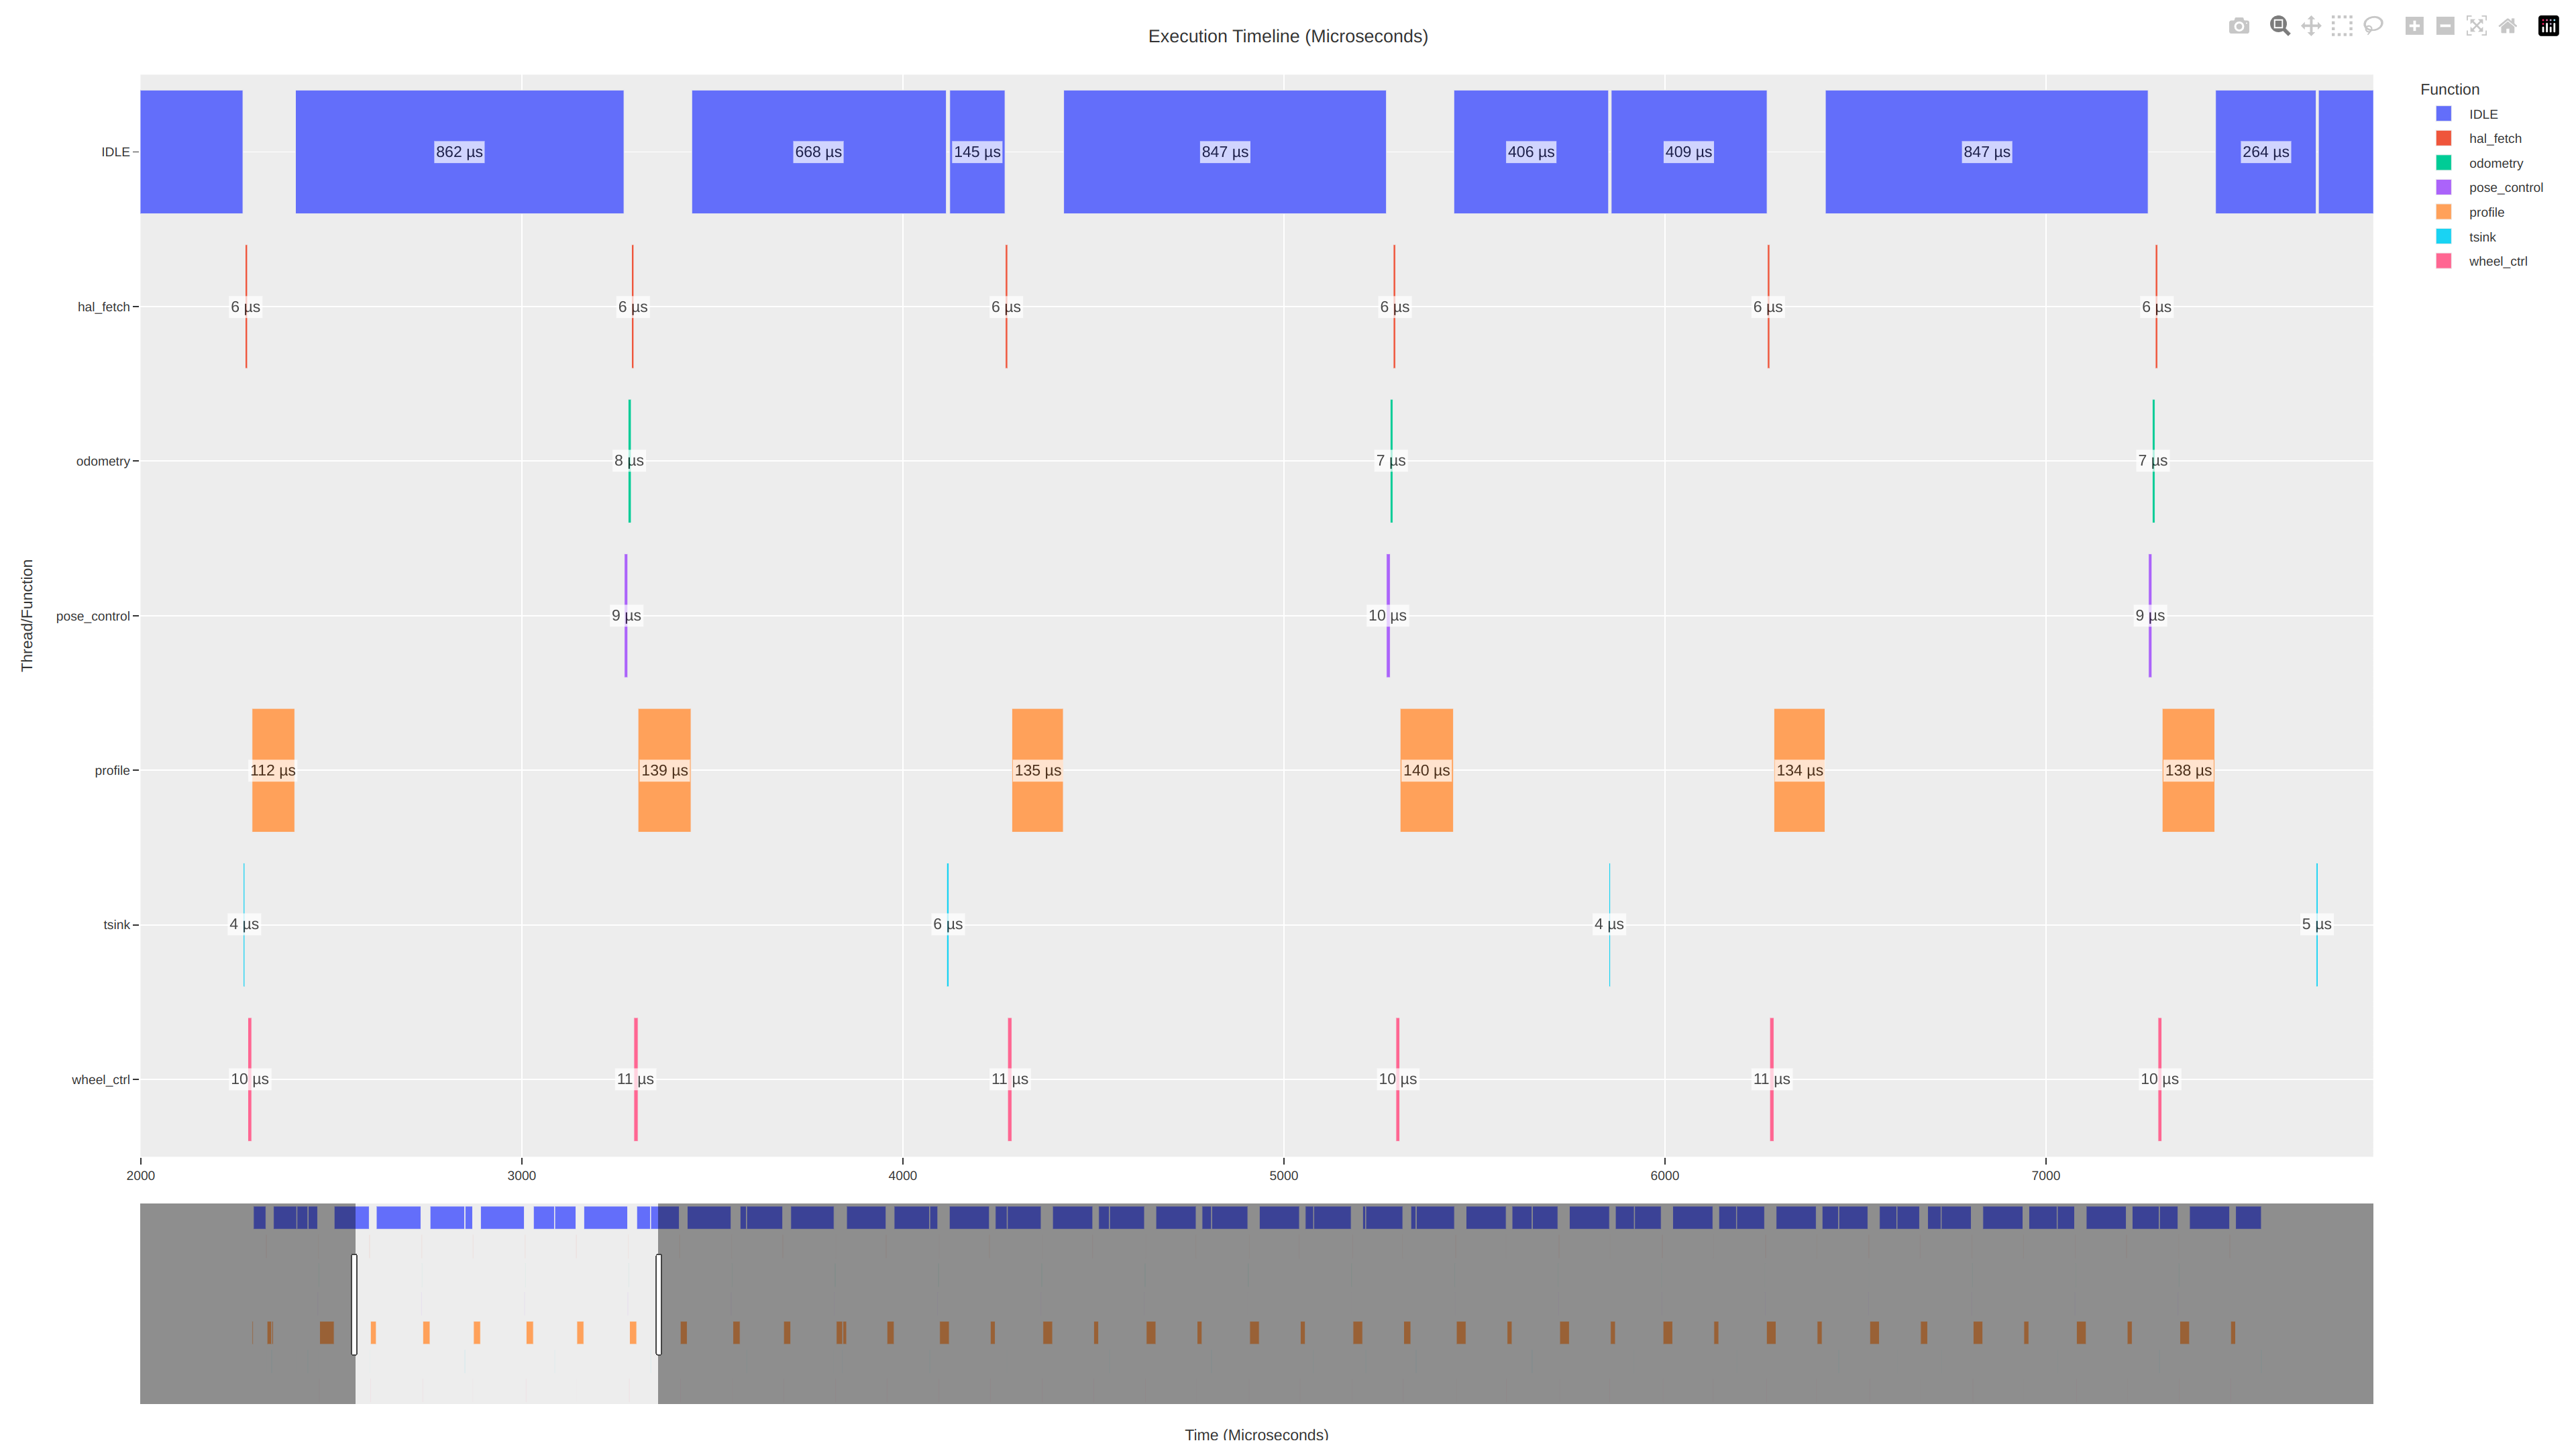
\includegraphics[width=1\textwidth]{assets/freertos_profiling_1000hz_ausschnitt}
    \caption{Visualisierung der Echtzeit-Statistik mit 1000 Hz (Ausschnitt)
    unter FreeRTOS}
\end{figure}

Wie in der Grafik illustriert, kann das Regelungssystem, dessen Tasks und
zugrundeliegende Kommunikation mittels FreeRTOS-APIs besonders schlank sind und
auf minimalen Overhead optimiert wurden, problemlos mit $1000\,\text{Hz}$
betrieben werden. Die Tasks werden rhythmisch und auch deterministisch jeweils
mit den vorgegebenen Frequenzen ausgeführt -- stets zum gleichen relativen
Zeitpunkt zueinander.

\begin{figure}[H]
    \centering
    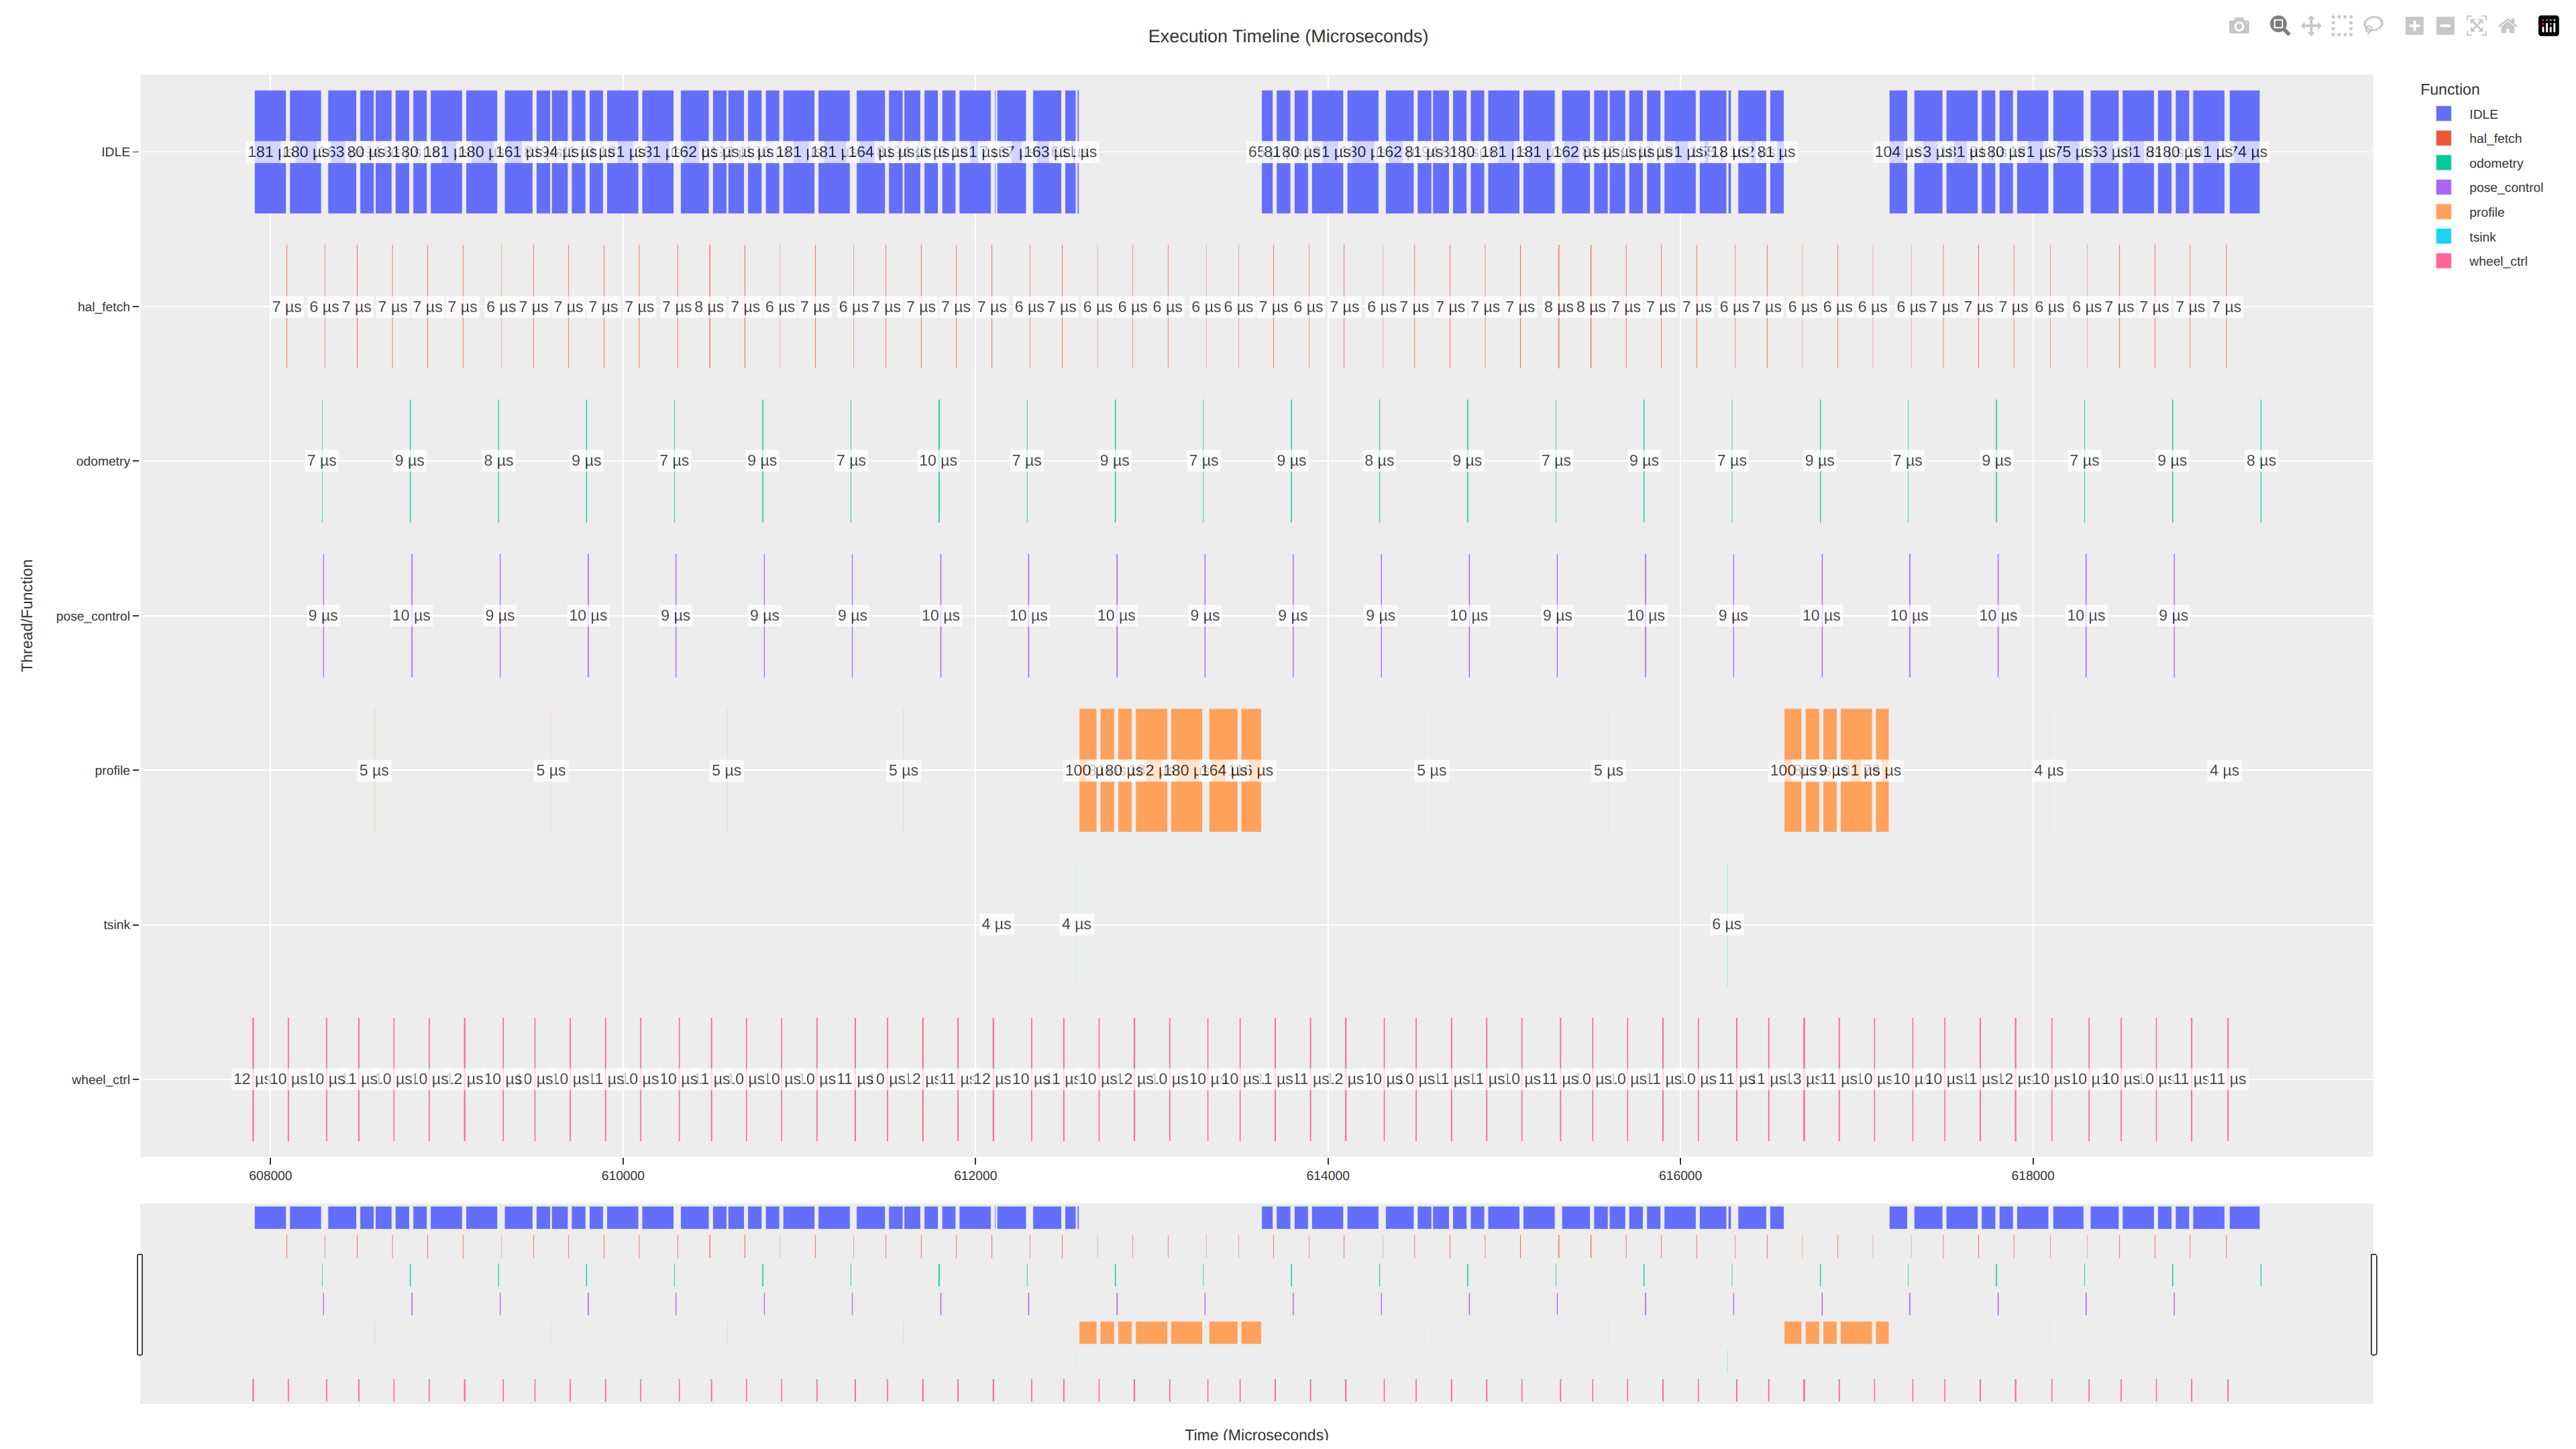
\includegraphics[width=1\textwidth]{assets/freertos_profiling_5000hz}
    \caption{Visualisierung der Echtzeit-Statistik mit 5000 Hz unter FreeRTOS}
\end{figure}

\begin{figure}[H]
    \centering
    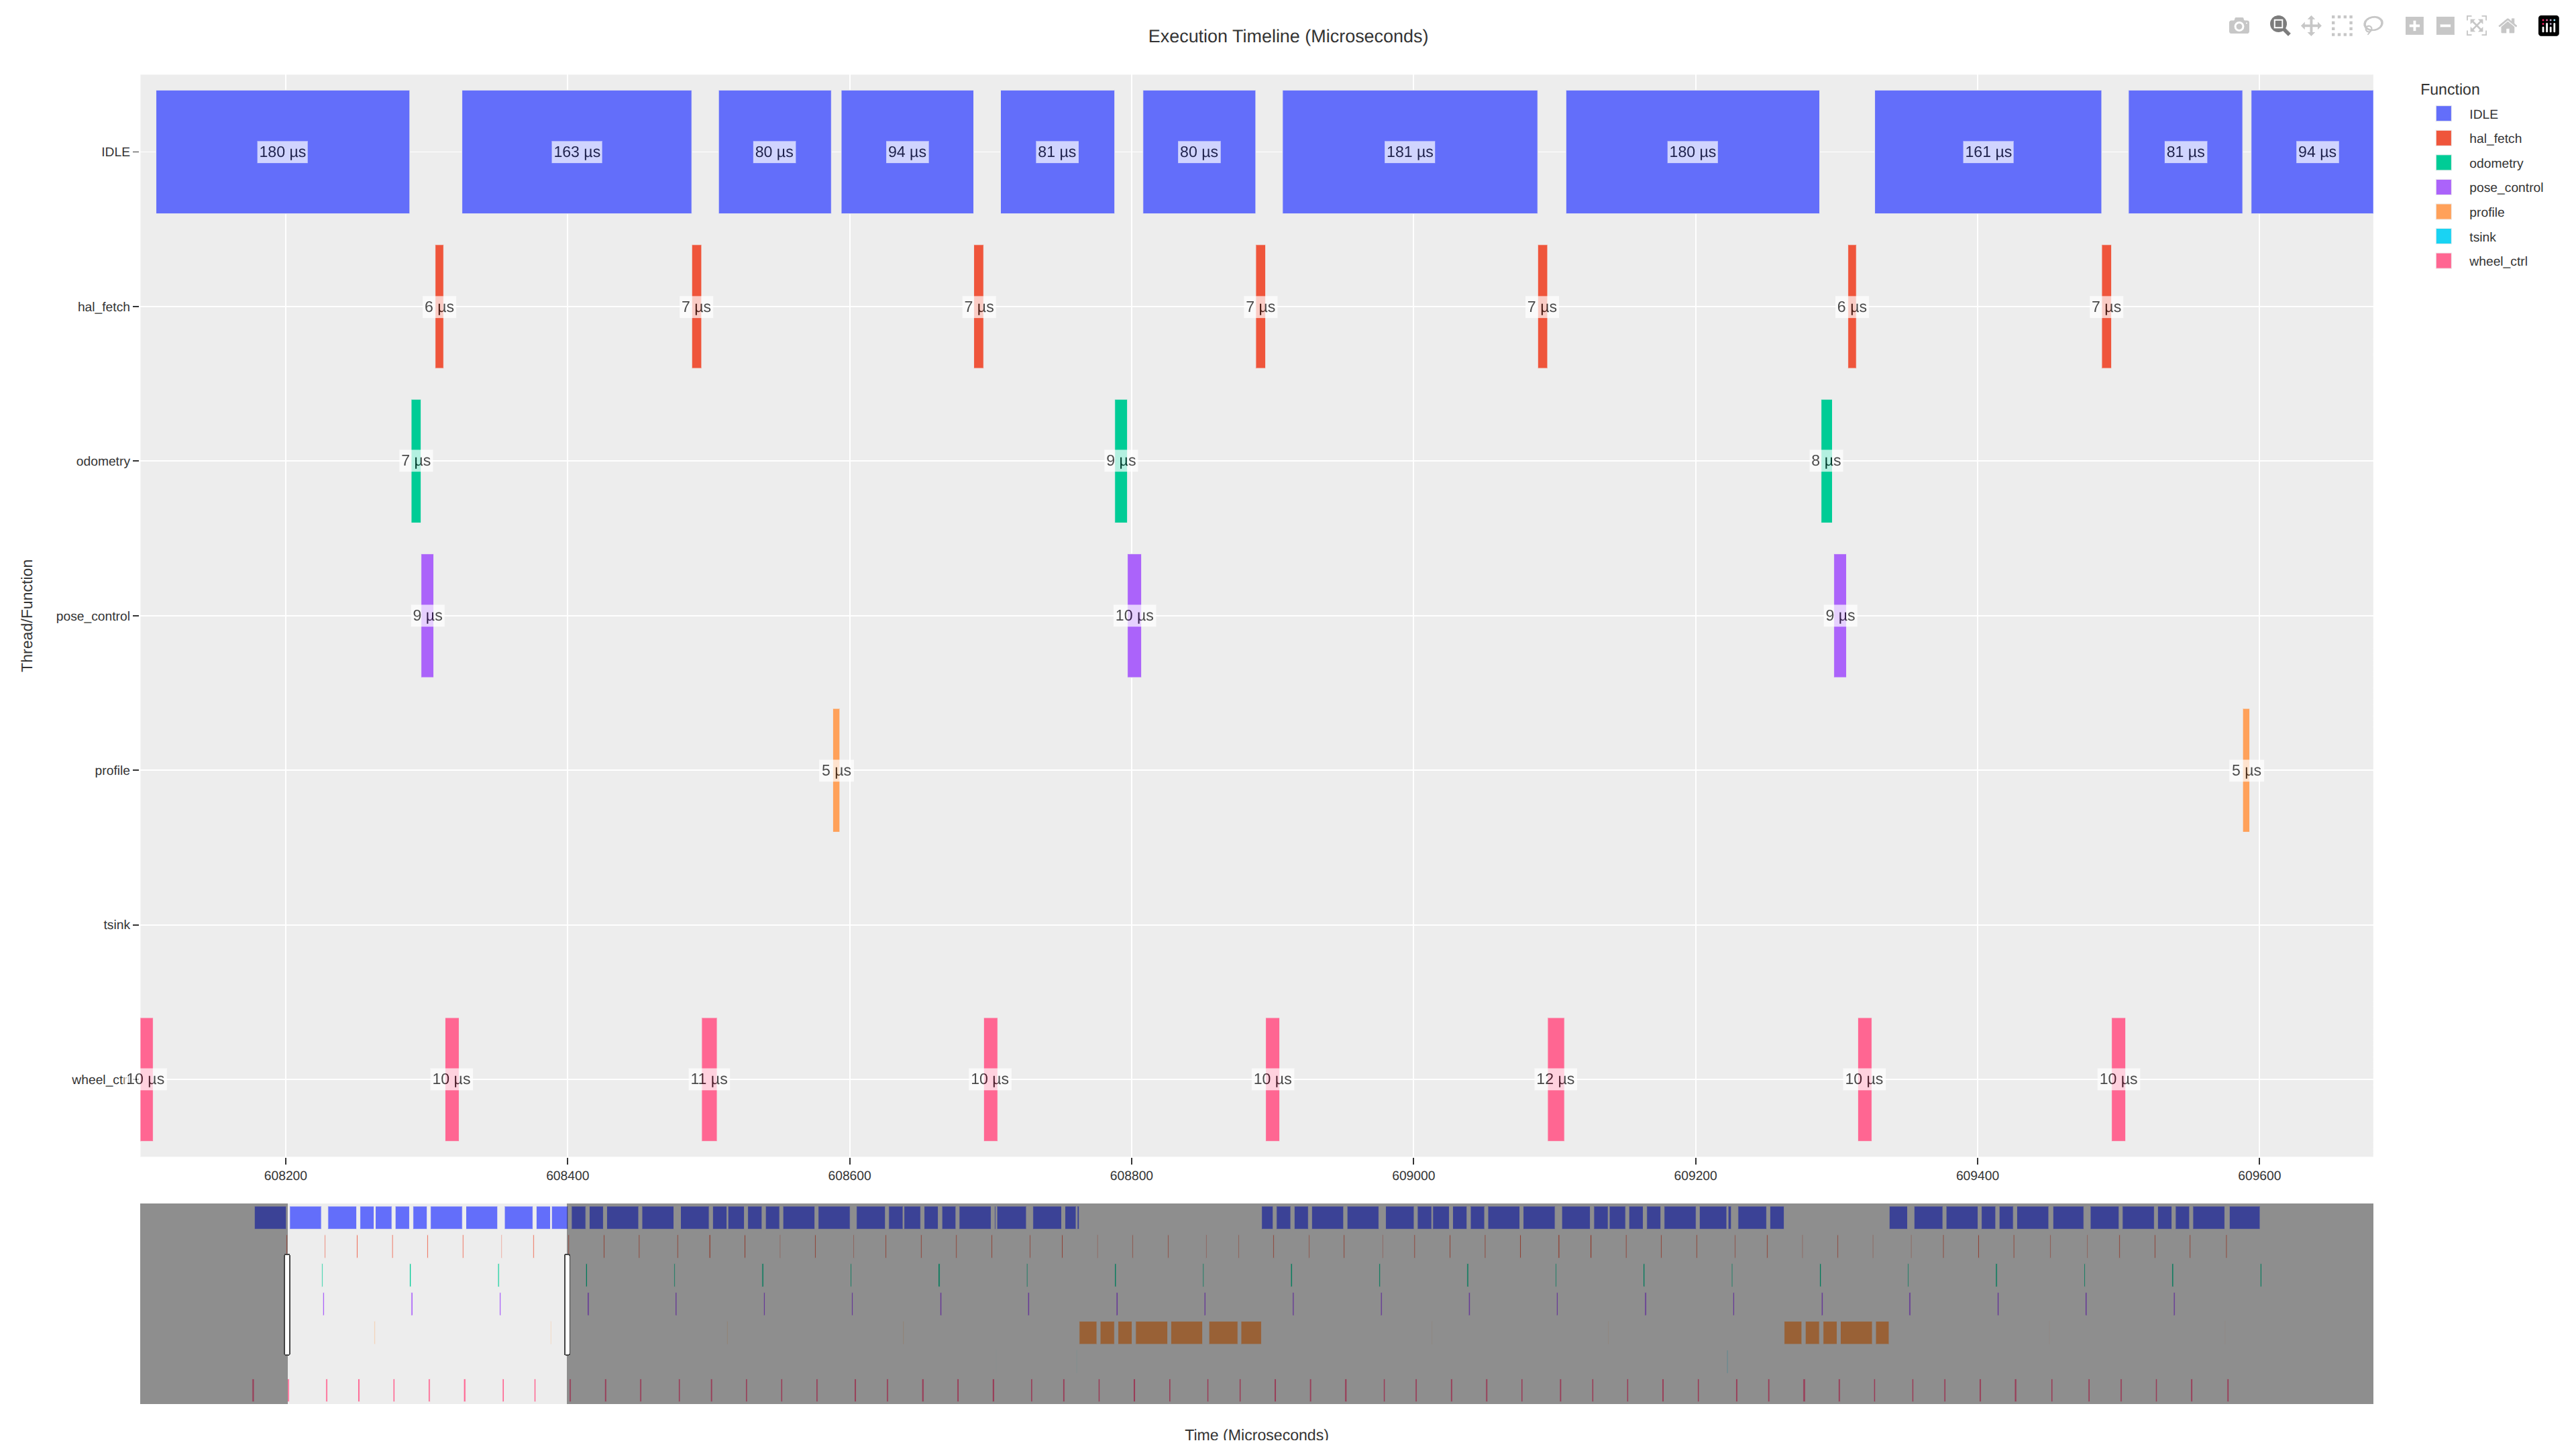
\includegraphics[width=1\textwidth]{assets/freertos_profiling_5000hz_ausschnitt}
    \caption{Visualisierung der Echtzeit-Statistik mit 5000 Hz (Ausschnitt)
    unter FreeRTOS}
\end{figure}

Bei einer $\textbf{5000\,\text{Hz}|2000\,\text{Hz}}$-Reglerkonfiguration führt
der Scheduler die Kontextwechsel weiterhin zuverlässig aus. Die Funktionen
werden korrekt alle $200\,\mu\text{s}$ bzw. $500\,\mu\text{s}$ aufgerufen,
obwohl das Profiling-Verfahren für diese Frequenzen nicht ausgelegt ist und den
Zwischenpuffer stets überläuft. Das System verbleibt bei diesen Frequenzen
größtenteils ebenfalls im Leerlauf.

\begin{code}
\begin{minted}{cpp}
IDLE 1 0
profile 2 1
profile 25 0
IDLE 27 1
IDLE 88 0
hal_fetch 89 1
hal_fetch 95 0
wheel_ctrl 96 1     << Start einer Iteration
wheel_ctrl 106 0
IDLE 107 1
IDLE 288 0
odometry 289 1      << Start einer Iteration
odometry 296 0
pose_control 297 1
pose_control 306 0
hal_fetch 307 1
hal_fetch 313 0
wheel_ctrl 313 1    << nach etwa 200 us zur vorherigen Iteration
...
odometry 788 1      << nach etwa 500 us zur vorherigen Iteration
\end{minted}
    \captionof{listing}{Profiling-Daten bei 5000|2000Hz}
\end{code}

\begin{figure}[H]
    \centering
    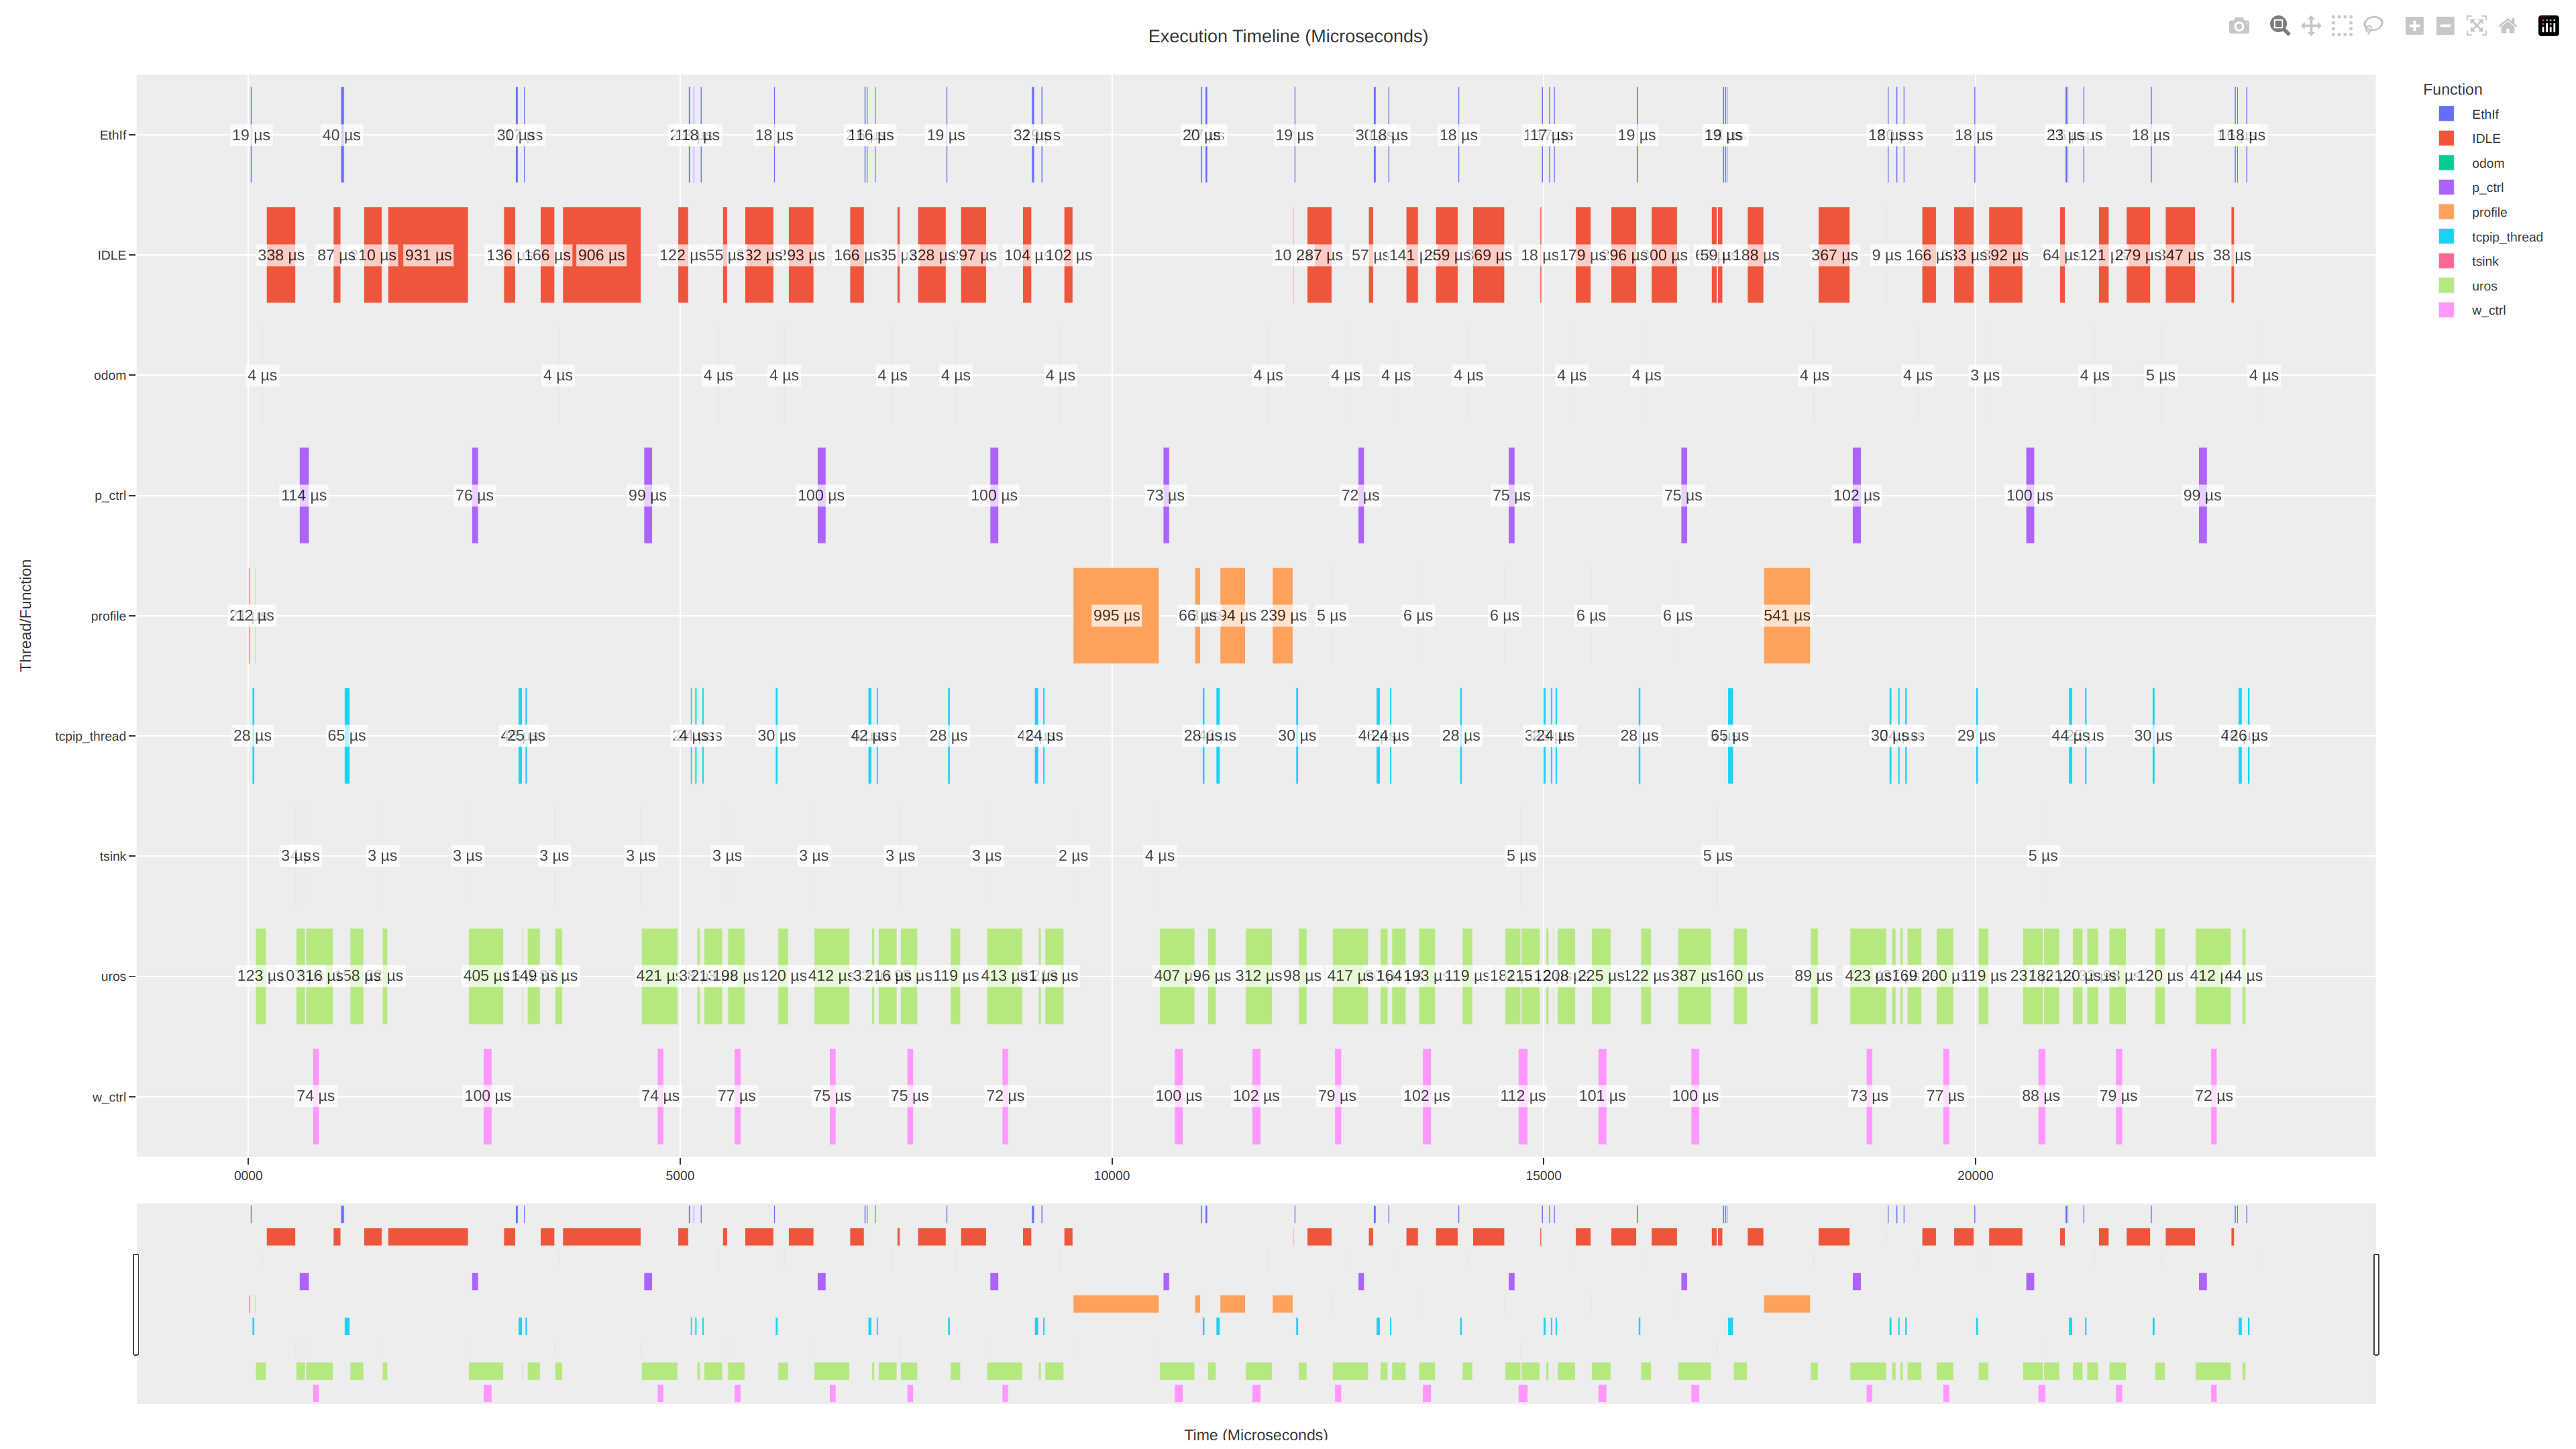
\includegraphics[width=1\textwidth]{assets/micro_ros_profiling_1000hz}
    \caption{Visualisierung der Echtzeit-Statistik mit 1000 Hz unter Micro-ROS}
\end{figure}

\begin{figure}[H]
    \centering
    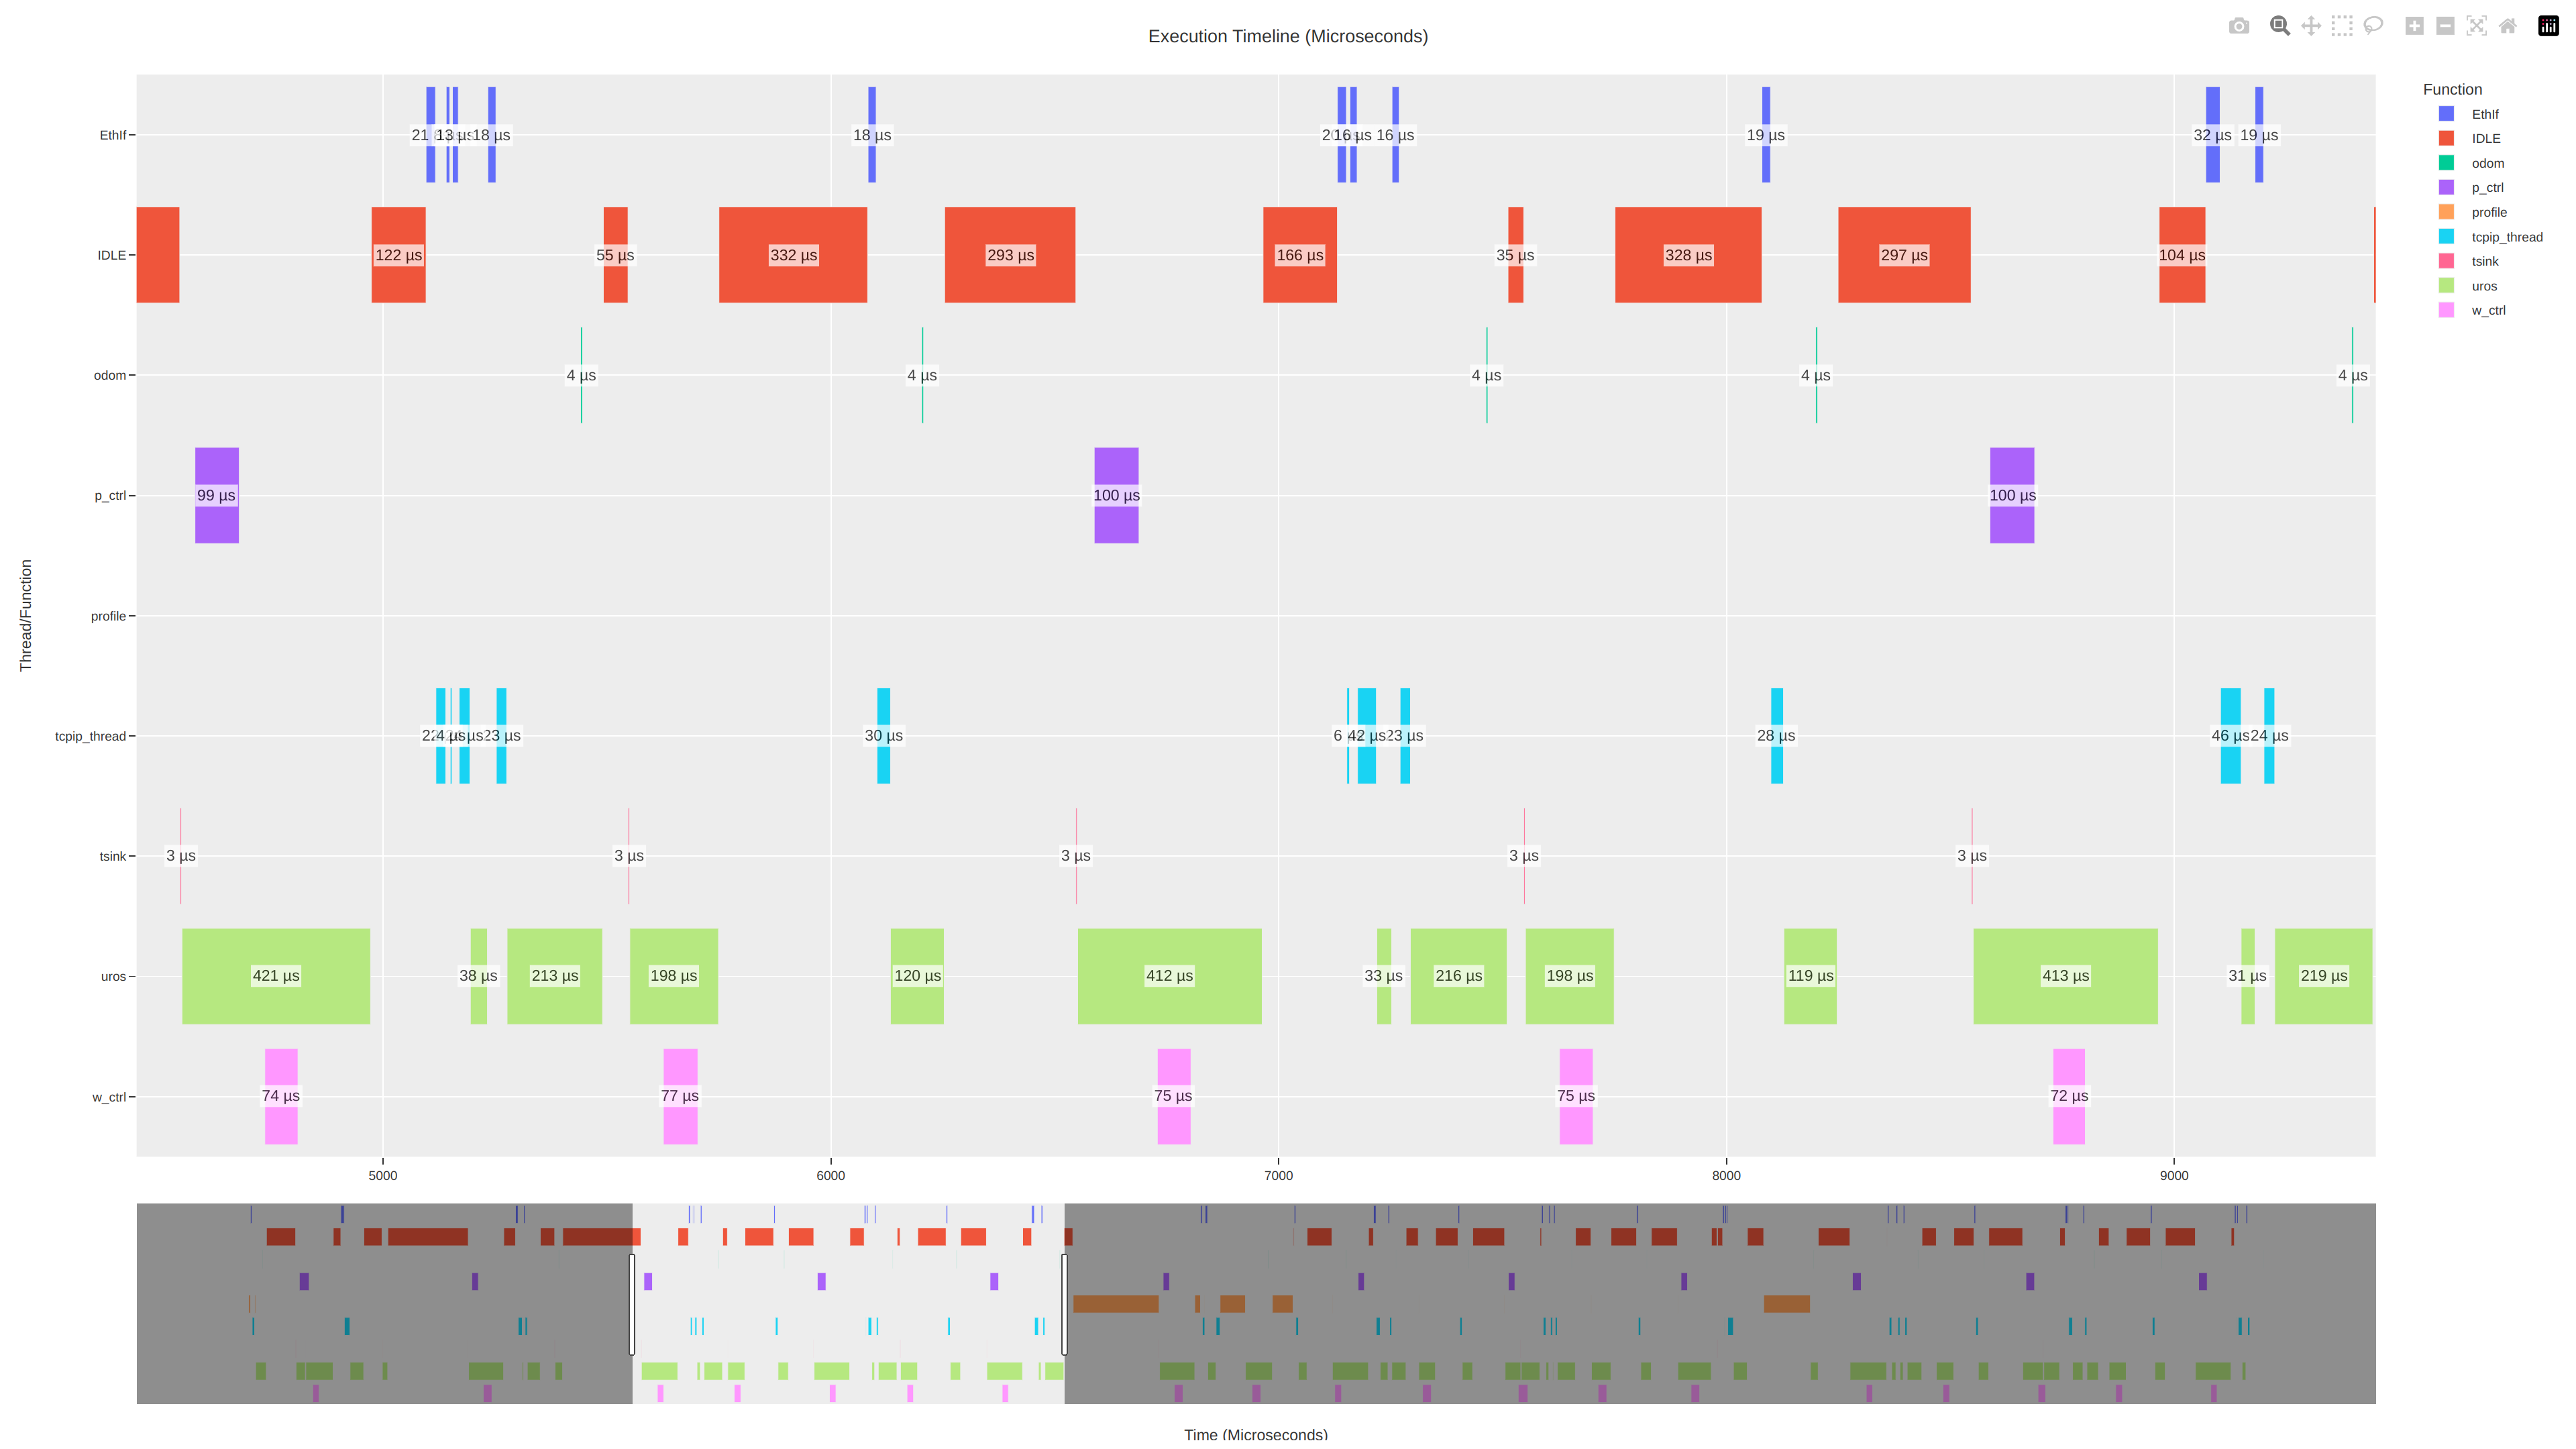
\includegraphics[width=1\textwidth]{assets/micro_ros_profiling_1000hz_ausschnitt}
    \caption{Visualisierung der Echtzeit-Statistik mit 1000 Hz (Ausschnitt)
    unter Micro-ROS}
\end{figure}

Micro-ROS erreichte die angestrebte Sollfrequenz von $1000\,\text{Hz}$ nicht und
wies stattdessen Schwankungen zwischen $910\,\text{Hz}$ und $980\,\text{Hz}$
auf. Dies lässt sich vermutlich auf zwei Hauptfaktoren zurückführen: Erstens
wird die maximal erreichbare Frequenz durch die Integration der zusätzlichen
Middleware beeinflusst -- konkret XRCE-DDS bei Micro-ROS und standardmäßig Fast
DDS bei ROS2, deren Performance und Konfiguration eine entscheidende Rolle
spielen \cite{ROS_Performance2019}. Zweitens verursacht der inhärente Overhead
des ROS/Micro-ROS-Stacks selbst signifikante Latenzen, denn jedes Datenpaket
durchläuft zwingend das ROS-Framework bzw. den Linux-Host (Mikrocontroller
$\leftrightarrow$ Host), im Gegensatz zu FreeRTOS-Implementierung, bei der der
komplette Datenaustausch intern erfolgt.

\subsubsection{Dauer von Regelungsfunktionen}

Aus den Profiling-Daten lässt sich ebenfalls folgender Vergleich zwischen den
beiden Implementierungen ableiten:

\begin{table}[h]
\centering
\begin{tabular}{|l|r|r|r|}
\hline
    \textbf{Name} & \textbf{Micro-ROS (\text{µs})} & \textbf{FreeRTOS (\text{µs})} & \textbf{Differenz (\text{µs})} \\ \hline
Odometrie & 6.780 (Ø:~3,74) & 6.256 (Ø:~6,84) & -524 \\ \hline
Posenregelung & 69.301 (Ø:~75,16) & 9.043 (Ø:~9,88) & 60.258 (Ø:~65,28) \\ \hline
Drehzahlregelung & 191.027 (Ø:~103,59) & 19.559 (Ø:~10,69) & 171.468 (Ø:~92,90) \\ \hline
\end{tabular}
\caption{Vergleich der Rechenzeiten zwischen Micro-ROS und FreeRTOS}
\end{table}

Die Implementierung ist auf beiden Plattformen größtenteils identisch, abgesehen
vom erwähnten Datenaustausch. Bei Micro-ROS müssen die Daten zusätzlich in einer
dedizierten Struktur mit Metadaten -- unter anderem einem Header mit Zeitstempel
in Sekunden und Nanosekunden -- umgewandelt werden. Bei FreeRTOS werden die
Daten direkt in die Warteschlange kopiert und beim Empfänger extrahiert.

Zusätzlich unterscheidet sich die FreeRTOS-Implementierung von Micro-ROS auch
dadurch, dass die Drehzahldaten nicht vom Drehzahlregler abgefragt und dann erst
an die Odometrie übergeben werden. Stattdessen übernimmt eine dedizierte
FreeRTOS-Task \mintinline{cpp}|hal_fetch| die Übertragung dieser Daten sowohl an
den Drehzahlregler als auch an die Odometrie (\ref{sec:freertos_tasks}). Dadurch
wird ein Teil des Overheads vom Drehzahlregler entkoppelt.

Zusammenfassend lässt sich feststellen, dass die Steuerungslogik an sich sowohl
unter Micro-ROS als auch unter FreeRTOS relativ wenig Rechenzeit benötigt,
sofern die Daten ordentlich gecacht sind und nicht bei jedem Zugriff aus dem RAM
geladen werden müssen. Unter FreeRTOS kann selbst bei deutlich höheren
Sollfrequenzen eine stabile Regelung erreicht werden. Dank des leistungsstarken
Mikrocontrollers in Kombination mit Cache-Nutzung und optimiertem Code befindet
sich das System auf beiden Plattformen überwiegend im Leerlauf.
